\chapter{Options pricing formula for American options in jump-diffusion dynamics and an approximate solution to the free boundary}
\chaptermark{Jump-diffusion -- American options}
 
 	\section{The PIDE system for American options and its solution}
   Continuing on from the European options in the previous chapter, we will now construct the necessary PIDE systems required to solve the American options pricing formula when the underlying asset is subjected to jump-diffusion dynamics. The analysis will begin with the American put option under a general jump distribution followed by a special case for the type of distribution that the jumps are assumed to follow. We will then repeat this analysis for the American call option.
   
     \subsection{American put option in jump-diffusion dynamics}
     \label{sec:amerputJD}
     Suppose we define the operator $\L'$ to be same as~\eqref{eqn:PIDE} except with $r$, $q$, and $\sigma$ to be constant instead of functions in time. This yields for a function $v = v(x,t)$
   \begin{equation}
   	\label{eqn:PIDE2}
   	\begin{split}
   	\L'v(x,t) &= \fr{\pr v}{\pr t}(x,t) + \fr{1}{2}\sigma^2x^2\fr{\pr^2 v}{\pr x^2} + (r-q-\kappa\lambda)x\fr{\pr v}{\pr x}(x,t) - rv(x,t) \\
   	&{}\quad + \lambda\int_0^\infty (v(xy,t)-v(x,t))f(y) \, \d y = 0.
   	\end{split}
   \end{equation}
   Then the American put option pricing problem with an underlying asset governed by jump-diffusion dynamics requires us to find two functions $ v_{\text{a}}^{\text{put}} = v_{\text{a}}^{\text{put}}(x,t)$ and $S^* = S^*(t)$ such that
        \begin{equation}
        \label{eqn:amerputPIDE}
        \begin{split}
            &v_{\text{a}}^{\text{put}}(x,T) = \max(K-x,0), \quad x \geq 0, \\
            &v_{\text{a}}^{\text{put}}(x,t) = K-x, \quad 0 \leq t < T \enskip \text{and} \enskip 0 \leq x < S^*(t), \\
            &\mathscr{L'}v_{\text{a}}^{\text{put}}(x,t) = 0, \quad 0 \leq t < T \enskip \text{and} \enskip x > S^*(t),
        \end{split}
    \end{equation}
    and at $x = S^*(t)$, the following smooth pasting conditions are satisfied:
    	\begin{equation}
    		\label{eqn:amerputPIDEsmc}
    		v_{\text{a}}^{\text{put}}(S^*(t),t) = K - S^*(t), \quad \fr{\pr v_{\text{a}}^{\text{put}}}{\pr x}(S^*(t),t) = -1.
    	\end{equation}
    	We now proceed to create an inhomogeneous PIDE system similar to \eqref{eqn:amerput} -- \eqref{eqn:amerputpasting}. We only need to analyze the region $0 \leq x < S^*(t)$ since we know for $x > S^*(t)$ that $\L' v_{\text{a}}^{\text{put}} = 0$. Applying the operator $\L'$ to $v_{\text{a}}^{\text{put}}$ for $0 \leq x < S^*(t)$ gives us
        \begin{align*}
            \L'v_{\text{a}}^{\text{put}}(x,t) &= -rK + (q+\kappa\lambda)x + \lambda\int_0^\infty \left( v_{\text{a}}^{\text{put}}(xy,t) - (K-x)\right)f(y) \, \d y \\
            &= -K(r+\lambda) + x(q + \lambda(\kappa+1)) + \lambda\int_0^\infty v_{\text{a}}^{\text{put}}(xy,t) \, \d y.
        \end{align*}
    The remaining integral needs to be dealt with carefully. This is because the value of $y$ can affect the value of $v_{\text{a}}^{\text{put}}(xy,t)$, thus changing whether we are in the continuation region or exercise/stopping region.
    Since the two possible cases are $0 \leq xy < S^*(t)$ and $xy > S^*(t)$, the critical value in terms of $y$ is $y = S^*(t)/x$. This means we have to split the integral into two regions giving
        \begin{align*}
            \L'v_{\text{a}}^{\text{put}}(x,t) &= -K(r+\lambda) + x(q + \lambda(\kappa+1)) + \lambda\int_0^\infty v_{\text{a}}^{\text{put}}(xy,t) \, \d y \\
            &= -K(r+\lambda) + x(q+\lambda(\kappa+1)) + \lambda\bigg( \int_0^{S^*(t)/x} v_{\text{a}}^{\text{put}}(xy,t)f(y) \, \d y \\
            &{} \quad + \int_{S^*(t)/x}^\infty v_{\text{a}}^{\text{put}}(xy,t)f(y) \, \d y \bigg) \\
            &= -K(r+\lambda) + x(q+\lambda(\kappa+1)) + \lambda\bigg( \int_0^{S^*(t)/x} (K - xy)f(y) \, \d y \\
            &{} \quad+ \int_{S^*(t)/x}^\infty v_{\text{a}}^{\text{put}}(xy,t)f(y) \, \d y \bigg),
        \end{align*}
    where we replaced $v_{\text{a}}^{\text{put}}(xy,t)$ with $K-xy$  for the first integral on the right-hand side since we are in the region $0 \leq y < S^*(t)/x$.
    We now split that same first integral on the right-hand side to get
        \begin{align*}
            \L'v_{\text{a}}^{\text{put}}(x,t) &= -K(r+\lambda) + x(q+\lambda(\kappa+1)) + \lambda\bigg( \int_0^\infty (K-xy)f(y) \, \d y  \\
            &\quad - \int_{S^*(t)/x}^\infty (K-xy)f(y) \, \d y + \int_{S^*(t)/x}^\infty v_{\text{a}}^{\text{put}}(xy,t)f(y) \, \d y \bigg)
        \end{align*}
  We know that $\kappa = \E[Y-1]$. Furthermore, we use the fact that
    $\lambda$ can be written as $\lambda\int_0^\infty f(y) \, \d y$ since $\int_0^\infty f(y) \, \d y=1$ and this simplifies our expression to
      \begin{align*}
          \L'v_{\text{a}}^{\text{put}}(x,t) &= -rK + qx + \lambda \int_{S^*(t)/x}^\infty \left(v_{\text{a}}^{\text{put}}(xy,t) - (K-xy)\right)f(y) \,\d y,
      \end{align*}
    for $0 < x < S^*(t)$. Now we create the inhomogeneous PIDE by simply appending a Heaviside function to account for
    $x > S^*(t)$ as we did for Eq.~\eqref{eqn:amerput}--\eqref{eqn:amerputpasting}, which reformulates our problem to the following system
      \begin{align}
          \label{eqn:amerPIDE}
          \L'v_{\text{a}}^{\text{put}}(x,t) = g_p(x,t)&, \enskip x \geq 0, \enskip x \neq S^*(t), \enskip 0 \leq t < T \\
          \label{eqn:amerPut}
          v_{\text{a}}^{\text{put}}(x,T) =  \max(K - x,0) &, \enskip x \geq 0, \enskip 0 \leq t < T \\
          \label{eqn:amerPasting}
          v_{\text{a}}^{\text{put}}(S^*(t),t) = K - S^*(t), \enskip &\fr{\pr v_{\text{a}}^{\text{put}}}{\pr x}(S^*(t),t) = -1, \enskip 0 \leq t < T,
      \end{align}
    where
      \begin{equation}
        \label{eqn:g}
        g_p(x,t) = \left(-rK + qx + \lambda \int_{S^*(t)/x}^\infty \left(v_{\text{a}}^{\text{put}}(xy,t) - (K-xy)\right)f(y) \,\d y \right)H(S^*(t)-x).
      \end{equation}
This PIDE system~\eqref{eqn:amerPIDE}--\eqref{eqn:amerPasting} is similar to~\eqref{eqn:amerput}--\eqref{eqn:amerputpasting} except now the model has been adjusted to accommodate for the presence of jumps. However, if we set $\lambda = 0$ which equates to having no jumps in the underlying asset dynamics, we would recover the standard diffusion PDE system for an American put.

To proceed with solving this system, we take the Mellin transform of \eqref{eqn:amerPIDE} with respect to $x$ and get
      \begin{equation}
      	  \label{eqn:PIDEODEamer}
        \fr{\pr \tilde{ v}_{\text{a}}^{\text{put}}}{\pr t}(\xi,t) - \left(p_\lambda(\xi) - \lambda\E[Y^{-\xi}]\right)\tilde{ v}_{\text{a}}^{\text{put}}(\xi,t) = \tilde{g}(\xi,t).
      \end{equation}
    with
      \begin{equation*}
        p_\lambda(\xi) = r + \lambda + \left(r - q -\kappa\lambda - \fr{\sigma^2}{2}\right)\xi - \fr{\sigma^2}{2}\xi^2,
      \end{equation*}
    and we leave the Mellin transform of $g(x,t)$ as it is without further computation. Notice how~\eqref{eqn:PIDEODEamer} is almost identical in form to~\eqref{eqn:PIDEODE} except that we are left with an additional function of $\xi$ and $t$ on the right-hand side. Furthermore, the expression for $p_\lambda$ here is the exact same as~\eqref{eqn:pMellin}. Thus we have an inhomogeneous linear ODE in $t$. Solving~\eqref{eqn:PIDEODEamer} by using an integrating factor $e^{-\left(p_\lambda(\xi) -\lambda\E[Y^{-\xi}]\right)(u-t)}$ and subject to a final condition at $u=T$ will yield
      $$
        \tilde{v}_{\text{a}}^{\text{put}}(\xi,t) = \tilde{ v}_{\text{a}}^{\text{put}}(\xi,T)e^{-\left(p_\lambda(\xi) -\lambda\E[Y^{-\xi}]\right)(T-t)} - \int_t^T e^{-\left(p_\lambda(\xi) -\lambda\E[Y^{-\xi}]\right)(u-t)}\tilde{g}_p(\xi,u) \, \d u.
      $$
      Recognising that $\tilde{ v}_{\text{a}}^{\text{put}}(\xi,T)$ is the Mellin transform of $v_{\text{a}}^{\text{put}}(\xi,T) = \max(K-x,0)$, we replace $\tilde{ v}_{\text{a}}^{\text{put}}(\xi,T)$ with $\tilde \phi_{\text{put}}(\xi)$ and obtain
       $$
        \tilde{ v}_{\text{a}}^{\text{put}}(\xi,t) = \tilde \phi_{\text{put}}(\xi)e^{-\left(p_\lambda(\xi) -\lambda\E[Y^{-\xi}]\right)(T-t)} - \int_t^T e^{-\left(p_\lambda(\xi) -\lambda\E[Y^{-\xi}]\right)(u-t)}\tilde{g}_p(\xi,u) \, \d u.
      $$
    Using the results from chapters 2 and 3, we take the inverse Mellin transform of both sides to obtain
      $$
       v_{\text{a}}^{\text{put}}(x,t) = (v_\lambda^{\text{put}}(\cdot,t) \ast \J(\cdot, t, T))(x)
        - \M^{-1}\left\{ \int_t^T e^{-\left(p_\lambda(\xi) -\lambda\E[Y^{-\xi}]\right)(u-t)}\tilde{g}_p(\xi,u) \, \d u \right\},
      $$
    where $\M^{-1}$ is the inverse Mellin operator, $v_\lambda^{\text{put}}$ = $v_\text{e}^{\text{put}}|_{r=r+\lambda,q=q+\lambda+\kappa\lambda}$ using the expression for $v_\text{e}^{\text{put}}$ from~\eqref{eqn:EUput}, $\J$ is the function
      \begin{equation}
      		\label{eqn:Jnew}
        \J(x,t,u) = \sum\limits_{n=0}^\infty \fr{(\lambda(u-t))^n}{n!}F_n(x),
      \end{equation}
    with $F_n$ defined in~\eqref{eqn:Fn}. We could have reused the definition of $\J$ from~\eqref{eqn:jumpGeneral}, but here we require a third argument for $\J$ that was not necessary in the European case.
    As~\eqref{eqn:optionJump} is for a European option with a general payoff, we can apply the result for a put option payoff and simplify the convolution term above to be
      $$
        (v_\lambda^{\text{put}}(\cdot,t) \ast \J(\cdot, t, T))(x) = v_{\text{e}}^{\text{put}}(x,t),
      $$
    so all that remains is to evaluate the remaining integral. To make the calculation a bit clearer, we will use
    	$$
    		e^{-\left(p_\lambda(\xi) -\lambda\E[Y^{-\xi}]\right)(u-t)} = \tilde{F}(\xi,u)
    	$$
    	for ease of notation. Using the Convolution theorem, the integral inverts to
      \begin{align*}
          \M^{-1}\left\{ \int_t^T \tilde{F}(\xi,u)\tilde{g}_p(\xi,u) \, \d u \right\} &=
          \int_t^T \M^{-1}\left\{\tilde{F}(\xi,u)\tilde{g}_p(\xi,u)\right\} \,\d u \\
          &= \int_t^T (F(\cdot,u)\ast g_p(\cdot,u))(x) \, \d u \\
          &= \int_t^T \int_0^\infty \fr{1}{z}F\left(\fr{x}{z},u\right)g_p(z,u) \, \d z \, \d u,
        \end{align*}
        where $F$ and $g$ are the inverse Mellin transforms of $\tilde F$ and $\tilde g$, respectively. We have purposefully expanded the convolution term to its integral form as this makes the next step much easier to see. The point of introducing $\tilde F$ is because, upon inversion, this term itself is another convolution. That is,
        \begin{align*}
        	F\left(\fr{x}{z},u\right) &= \M^{-1}\left\{\tilde{F}(\xi,u)\right\} = \M^{-1}\left\{e^{-\left(p_\lambda(\xi) -\lambda\E[Y^{-\xi}]\right)(u-t)}\right\} \\
        	&= (\K_\lambda(\cdot,t,u)\ast \J(\cdot,t,u))\left(\fr{x}{z}\right) = \int_0^\infty \fr{1}{w}\J(w,t,u)\K_\lambda\left( \fr{x}{zw},t,u \right) \, \d w,
        \end{align*}
        where we used the inverse Mellin transform of $e^{\lambda\E[Y^{-\xi}](u-t)}$ from~\eqref{eqn:JMellin} and $e^{-p_\lambda(\xi)(u-t)}$ from~\eqref{eqn:optionConv}, and also $\mathscr{K}_\lambda$ given in~\eqref{eqn:shiftKernel}. Thus,
        	\begin{align*}
        		\M^{-1}\left\{ \int_t^T \tilde{F}(\xi,u)\tilde{g}_p(\xi,u) \, \d u \right\} &= \int_t^T \int_0^\infty \int_0^\infty \fr{1}{z}g_p(z,u) \fr{1}{w}\J(w,t,u) \\
        		 & \qquad \qquad \times \K_\lambda\left(\fr{x}{zw},t,u\right) \, \d w \, \d z \, \d u,
        	\end{align*}
        	and our American put option pricing formula under jump-diffusion dynamics is 
        	\begin{equation}
        		\label{eqn:amerJumpPut}
        		v_{\text{a}}^{\text{put}}(x,t) = v_{\text{e}}^{\text{put}}(x,t) + \int_t^T \int_0^\infty \int_0^\infty \fr{1}{z}g_p(z,u) \fr{1}{w}\J(w,t,u)\K_\lambda\left(\fr{x}{zw},t,u\right) \, \d w \, \d z \, \d u.
        	\end{equation}
        	This is very similar in form to~\eqref{eqn:americanput} but with the triple integral on the right-hand side in lieu of a single integral representing the early exercise premium that is inherent for American options.
        	
        	\subsection{Example: lognormally distributed jumps for an American put option}
        	As a special case for the American put option, we will assume that the underlying asset follows lognormally distributed jump dynamics. This will allow us to evaluate a few of the integrals that appear in~\eqref{eqn:amerJumpPut}. As a preparatory step, we will first denote the triple integral in~\eqref{eqn:amerJumpPut} by $I$. Then using the expression for $g_p$ from~\eqref{eqn:g}, we see that
        	\begin{align*}
        		I &= -rK \int_t^T\int_0^\infty\int_0^{S^*(u)}\fr{1}{w}\J(w,t,u)\fr{1}{z}\K_\lambda\left( \fr{x}{zw},t,u \right) \, \d z \, \d w \, \d u \\
        		& {} \quad + q \int_t^T\int_0^\infty\int_0^{S^*(u)}\fr{1}{w}\J(w,t,u)\K_\lambda\left( \fr{x}{zw},t,u \right) \, \d z \, \d w \, \d u \\
        		& {} \quad + \int_t^T\int_0^\infty\int_0^{S^*(u)} \fr{1}{w}\J(w,t,u)\fr{1}{z}\K_\lambda\left( \fr{z}{w},t,u \right) \\
        		&{} \quad \quad \times  \lambda \int_{S^*(u)/z}^\infty \left( v_{\text{a}}^{\text{put}}(zy,t) - (K-zy) \right)f(y) \, \d y \, \d z \, \d w \, \d u \\
        		& = I_1 + I_2 + I_3,
        	\end{align*}
        	where we had to swap the integrals with respect to $w$ and $z$ in order to simplify the Heaviside function that appears in $g_p$. Each of these integrals will be investigated separately to see if they can be simplified. For $I_1$, we will make use of eq.~\eqref{eqn:jump11} for $\J$ and the first identity in~\eqref{eqn:shiftKernel} for $\K_\lambda$ (assuming time-constant functions for $r$, $q$, and $\sigma$) to get
        		\begin{align*}
        			I_1 &= -rK\int_t^T \fr{e^{(r+\lambda)(u-t)}}{\sigma\sqrt{u-t}} \int_0^\infty\int_0^{S^*(u)} \fr{1}{w} \delta(w-1) \fr{1}{z} N'\left( z_{2\lambda}\left( \fr{x}{zw}, t, u \right) \right) \, \d z \, \d w \, \d u \\
        			& {}\quad -rK\int_t^T \fr{e^{(r+\lambda)(u-t)}}{\sigma\sqrt{u-t}} \ds\sum\limits_{n=1}^{\infty} \fr{(\lambda(u-t))^n}{n!\sqrt{n\sigma_Y^2}}\int_0^\infty \int_0^{S^*(u)} \fr{1}{zw}N'\left( \fr{\log w + n\mu_Y}{\sqrt{n\sigma_Y^2}} \right) \\
        			& {} \quad \quad \times N'\left( z_{2\lambda}\left( \fr{x}{zw}, t, u \right) \right) \, \d z \, \d w \, \d u \\
        			&= I_{1,a} + I_{1,b}.
        		\end{align*}
		For $I_{1,a}$, we swap the order of integration between $z$ and $w$ (constant limits with respect to each of these dummy variables) and using the well known result of $f(a) = \int_0^\infty \delta(x-a) f(x) \, \d x$ for $a > 0$ to obtain
        		$$
        			I_{1,a} = -rK\int_t^T \fr{e^{(r+\lambda)(u-t)}}{\sigma\sqrt{u-t}}\int_0^{S^*(u)} \fr{1}{z} N'\left( z_{2\lambda}\left( \fr{x}{z}, t, u \right) \right) \, \d z \, \d u.
        		$$
		Then we employ Lemma~\ref{lem:2a} and referring to~\eqref{eqn:z2lambda} for the complete expression of $z_{2\lambda}$, we can assign
			$$
				a = 0, \enskip b = S^*(u), \enskip a_1 = \fr{1}{\sqrt{n\sigma_Y^2 + \sigma^2(u-t)}}, \enskip
			b_1 = z_2\left( \fr{x}{z}, t, u \right),
			$$
		which then gives us
			\begin{align*}
				I_{1,a} &=  -rK\int_t^T e^{(r+\lambda)(u-t)}N\left(-z_{2\lambda}\left( \fr{x}{S^*(u)},t,u\right) \right) \, \d u.
			\end{align*}
			Unfortunately, the time integral cannot be solved analytically without prior knowledge of $S^*$ so it will be left unsimplified
		
        	For $I_{1,b}$, we once again swap the order of integration between $z$ and $w$. Then we make use of lemma~\ref{lem:1} because $z_{2\lambda}$ takes the form of a logarithmic function. In accordance to Lemma~\ref{lem:1}, we make the following declarations
        		$$
        			a_1 = \fr{1}{\sqrt{n\sigma_Y^2}}, \enskip b_1 = \fr{n\mu_Y}{\sqrt{n\sigma_Y^2}}, \enskip
        			a_2 = \fr{1}{\sigma\sqrt{u-t}}, \enskip b_2 = z_{2\lambda}\left( \fr{x}{z}, t, u\right),
        		$$
	and integrating with respect to $w$ leaves us with
			\begin{align*}
				I_{1,b} &= -rK  \int_t^T  \ds\sum\limits_{n=1}^{\infty} \fr{(\lambda(u-t))^n}{n!\sqrt{n\sigma_Y^2 + \sigma^2(u-t)}}  e^{(r+\lambda)(u-t)} \int_0^{S^*(u)} \fr{1}{z}  N\left(Z_n \left( \fr{x}{z},t,u  \right) \right) \,\d z \, \d u,
			\end{align*}
	where $Z_n$ is defined in~\eqref{eqn:zn}. To compute the integral with respect to $z$, we once again incorporate lemma~\ref{lem:2a} and set 
		$$
			a = 0, \enskip b = S^*(u), \enskip a_1 = \fr{1}{\sqrt{n\sigma_Y^2 + \sigma^2(u-t)}}, \enskip
			b_1 = Z_n\left( \fr{x}{z}, t, u \right),
		$$
		to obtain
		$$
			I_{1,b} = -rK  \int_t^T  \ds\sum\limits_{n=1}^{\infty} \fr{(\lambda(u-t))^n}{n!}  e^{(r+\lambda)(u-t)} N\left(- Z_n \left( \fr{x}{S^*(u)},t,u  \right) \right) \, \d u.
		$$
		Now adding $I_{1,a}$ and $I_{1,b}$ gives us the original integral $I_1$, and finally
		\begin{align}
			I_1 &= -rK\int_t^T e^{(r+\lambda)(u-t)}N\left(-z_{2\lambda}\left( \fr{x}{S^*(u)},t,u\right) \right) \, \d u \nonumber \\
			 &\quad -rK  \int_t^T  \ds\sum\limits_{n=1}^{\infty} \fr{(\lambda(u-t))^n}{n!}  e^{(r+\lambda)(u-t)} N\left(- Z_n \left( \fr{x}{S^*(u)},t,u  \right) \right) \, \d u \nonumber \\
			 &= -rK \ds\sum\limits_{n=0}^{\infty}\int_t^T  \fr{(\lambda(u-t))^n}{n!} e^{(r+\lambda)(u-t)} N\left(-Z_n \left( \fr{x}{S^*(u)},t,u  \right) \right) \, \d u, \label{eqn:I1put}
		\end{align}
		where after comparing $z_{2\lambda}$ and $Z_n$ (i.e., when $n=0$, $Z_0 = z_{2\lambda}$), the summation can actually encompass both terms with an extended summation index to $n=0$. This was not possible to do before as the original summation term that appears in $\J$ possessed a fraction that would have been undefined at $n=0$.
		
		We now give a similar treatment to $I_2$. Substituting~\eqref{eqn:jump11} for $\J$ but using the second identity for $\K_\lambda$ in~\eqref{eqn:shiftKernel} (again, assuming the functions $r$, $q$, and $\sigma$ are constant with respect to $t$), we find that
		\begin{align*}
        			I_2 &= -q\int_t^T \fr{e^{(r+\lambda)(u-t)}}{\sigma\sqrt{u-t}} \int_0^\infty\int_0^{S^*(u)} \fr{1}{w} \delta(w-1) N'\left( z_{2\lambda}\left( \fr{x}{zw}, t, u \right) \right) \, \d z \, \d w \, \d u \\
        			& {}\quad -q\int_t^T \fr{e^{(r+\lambda)(u-t)}}{\sigma\sqrt{u-t}} \ds\sum\limits_{n=1}^{\infty} \fr{(\lambda(u-t))^n}{n!\sqrt{n\sigma_Y^2}}\int_0^\infty \int_0^{S^*(u)} \fr{1}{w}N'\left( \fr{\log w + n\mu_Y}{\sqrt{n\sigma_Y^2}} \right) \\
        			& {} \quad \quad \times N'\left( z_{2\lambda}\left( \fr{x}{zw}, t, u \right) \right) \, \d z \, \d w \, \d u \\
        			&= I_{2,a} + I_{2,b}.
        		\end{align*}
		To calculate $I_{2,a}$, we swap the integrals with respect to $z$ and $w$ and using the properties of the Dirac delta function gives us
			$$
				I_{2,a} = qx\int_t^T \fr{e^{(q+\lambda+\kappa\lambda)(u-t)}}{\sigma\sqrt{u-t}}\int_0^{S^*(u)} N'\left( z_{1\lambda}\left( \fr{x}{z}, t, u \right) \right) \, \d z \, \d u.
			$$
		Then using the second result of Lemma~\ref{lem:2a} with
			$$
				a = 0, \enskip b = S^*(u), \enskip a_1 = \fr{1}{\sqrt{n\sigma_Y^2 + \sigma^2(u-t)}}, \enskip
			b_1 = z_1\left( \fr{x}{z}, t, u \right),
			$$
		the integral becomes
			$$
				I_{2,a} = qx\int_t^T e^{(q+\lambda+\kappa\lambda)(u-t)} N'\left(-z_{1\lambda}\left( \fr{x}{S^*(u)}, t, u \right) \right) \, \d z \, \d u.
			$$
		with $z_{1\lambda}$ from~\eqref{eqn:z1lambda}. Similarly for $I_{2,b}$, we apply the same procedure as we did for $I_{1,b}$ except when using lemma~\ref{lem:1}, we choose
			$$
        			a_1 = \fr{1}{\sqrt{n\sigma_Y^2}}, \enskip b_1 = \fr{n\mu_Y}{\sqrt{n\sigma_Y^2}}, \enskip
        			a_2 = \fr{1}{\sigma\sqrt{u-t}}, \enskip b_2 = z_{1\lambda}\left( \fr{x}{z}, t, u\right),
        		$$
	to get
			\begin{align*}
				I_{2,b} &= q  \int_t^T  \ds\sum\limits_{n=1}^{\infty} \fr{(\lambda(u-t))^n}{n!\sqrt{n\sigma_Y^2 + \sigma^2(u-t)}}  e^{(r+\lambda)(u-t)} \int_0^{S^*(u)} N\left( Z_n \left( \fr{x}{z},t,u  \right) \right) \,\d z \, \d u.
			\end{align*}
	To compute the remaining integral with respect to $z$, we once again have the aid of the second result from lemma~\ref{lem:2a} and set
			$$
				a = 0, \enskip b = S^*(u), \enskip a_1 = \fr{1}{\sqrt{n\sigma_Y^2 + \sigma^2(u-t)}}, \enskip
			b_1 = Z_n\left( \fr{x}{z}, t, u \right).
			$$
	Upon doing this, $I_{2,b}$ becomes
			$$
				I_{2,b} = qx  \int_t^T  \ds\sum\limits_{n=1}^{\infty} \fr{(\lambda(u-t))^n}{n!} e^{n\mu_Y + n\sigma_Y^2/2} e^{(q+\lambda + \kappa\lambda)(u-t)} N\left( -D_n \left( \fr{x}{S^*(u)},t,u  \right) \right) \, \d u,
			$$
	where we have defined a new function $D_n$ to be
			\begin{equation}
				\label{eqn:Dn}
				D_n(x,t,u) = \fr{\log x + n\mu_Y + n\sigma_Y^2 + (r-q-\kappa\lambda + \sigma^2/2)(u-t)}{\sqrt{n\sigma_Y^2 + \sigma^2(u-t)}}.
			\end{equation}
	Now like $I_1$, we can obtain $I_2$ by adding $I_{2,a}$ and $I_{2,b}$. In a similar manner to $I_2$, we notice that when $n=0$, $D_0 = z_{1\lambda}$. So then this leads to 
        	\begin{equation}
        		\label{eqn:I2put}
        		I_2 = qx  \ds\sum\limits_{n=0}^{\infty}\int_t^T   \fr{(\lambda(u-t))^n}{n!} e^{n\mu_Y + n\sigma_Y^2/2} e^{(q+\lambda + \kappa\lambda)(u-t)} N\left( -D_n \left( \fr{x}{S^*(u)},t,u  \right) \right) \, \d u.
        	\end{equation}
	The final integral, $I_3$, is probably the most difficult to simplify because it contains 4 integrals. Nevertheless, it is possible to manipulate this expression and reduce it down to 2 integrals which would undoubtedly help in alleviating some strain on any numerical computations. To start off, we first set
		$$
			F(z,u) = \lambda\int_{S^*(u)/z}^\infty  \left( v_{\text{a}}^{\text{put}}(zy,t) - (K-zy) \right)f(y) \, \d y,
		$$
	which corresponds to the innermost integral of $I_3$. Next we swap the order of integration between $z$ and $w$ to give
		$$
			I_3 = \int_t^T\int_0^{S^*(u)} \fr{F(z,u)}{z} \int_0^\infty  \fr{1}{w}\J(w,t,u)\K_\lambda\left( \fr{x}{zw},t,u \right) \, \d w \, \d z \, \d u. 
		$$
	Then by using $\J$ from~\eqref{eqn:jump11} for a lognormal distribution, the integral becomes
		\begin{align*}
			I_3 &= \int_t^T\int_0^{S^*(u)} \fr{F(z,u)}{z} \int_0^\infty  \fr{1}{w}\delta(w-1)\K_\lambda\left( \fr{x}{zw},t,u \right) \, \d w \, \d z \, \d u \\
			& \quad {} + \int_t^T\int_0^{S^*(u)} \fr{F(z,u)}{z} \int_0^\infty  \fr{1}{w}  \ds\sum\limits_{n=1}^{\infty} \fr{(\lambda(u-t))^n}{n!\sqrt{n\sigma_Y^2}} N'\left( \fr{\log w + n\mu_Y}{\sqrt{n\sigma_Y^2}} \right) \\
			&\quad \quad {} \times \K_\lambda\left( \fr{x}{zw},t,u \right) \, \d w \, \d z \, \d u \\
			&= I_{3,a} + I_{3,b}.
		\end{align*} 
	Evaluating $I_{3,a}$ results in
		\begin{align*}
			I_{3,a} &= \int_t^T \int_0^{S^*(u)} \fr{F(z,u)}{z}\K_\lambda\left( \fr{x}{z},t,u \right) \, \d z \, \d u \\
			&= \lambda  \int_t^T \int_0^{S^*(u)} \fr{1}{z}\K_\lambda\left( \fr{x}{z},t,u \right) \int_{S^*(u)/z}^\infty  \left( v_{\text{a}}^{\text{put}}(zy,t) - (K-zy) \right)f(y) \, \d y \, \d z \, \d u.
		\end{align*}
	The next step is to swap the order of integration between $y$ and $z$, but we must be careful because one of the limits depends $z$. From this we get
		$$
			I_{3,a} = \lambda  \int_t^T \int_1^\infty f(y) \int_{S^*(u)/y}^{S^*(u)} \fr{1}{z}\K_\lambda\left( \fr{x}{z},t,u \right)  \left( v_{\text{a}}^{\text{put}}(zy,t) - (K-zy) \right) \, \d z \, \d y \, \d u.
		$$
	Now we invoke a change of variables by letting $p = (zy)/S^*(u)$. This is so we can remove $S^*$ from the limits of integration. The substitution leads us to
		\begin{align*}
			I_{3,a} &=  \lambda  \int_t^T \int_1^\infty f(y) \int_1^y \fr{1}{p}\K_\lambda\left( \fr{xy}{S^*(u)p},t,u \right)  \\
			&\quad {} \times \left( v_{\text{a}}^{\text{put}}(S^*(u)p,t) - (K-S^*(u)p) \right) \, \d p \, \d y \, \d u.
		\end{align*}
	Now we reverse the order of integration between $p$ and $y$ and we see that
		\begin{align*}
			I_{3,a} &=  \lambda  \int_t^T \int_1^\infty \fr{1}{p} \left( v_{\text{a}}^{\text{put}}(S^*(u)p,t) - (K-S^*(u)p) \right)  \\
			&\quad {} \times \int_p^\infty f(y)\K_\lambda\left( \fr{xy}{S^*(u)p},t,u \right) \, \d y \, \d p \, \d u.
		\end{align*}
	Recalling the definition of $f$ for lognormally distributed jumps in~\eqref{eqn:LNPDF} and the first identity for $\K_\lambda$ in~\eqref{eqn:shiftKernel}, the integral expands to
		\begin{align*}
			I_{3,a} &=  \fr{\lambda}{\sigma_Y}  \int_t^T \fr{e^{(r+\lambda)(u-t)}}{\sigma\sqrt{u-t}} \int_1^\infty \fr{1}{p} \left( v_{\text{a}}^{\text{put}}(S^*(u)p,t) - (K-S^*(u)p) \right)  \\
			&\quad {} \times \int_p^\infty \fr{1}{y}N'\left( \fr{\log y - \mu_Y}{\sigma_Y} \right)N'\left( z_{2\lambda}\left( \fr{xy}{S^*(u)p}, t, u \right)\right) \, \d y \, \d p \, \d u 
		\end{align*}
		The innermost integral can be evaluated using lemma~\ref{lem:2b} and the associated variables be set to
		$$
			a_1 = \fr{1}{\sigma_Y}, \enskip b_1 = \fr{-\mu_Y}{\sigma_Y}, \enskip a_2 = \fr{-1}{\sigma\sqrt{u-t}}, \enskip
			b_2 = z_{2\lambda}\left( \fr{x}{S^*(u)p}, t, u \right), \enskip c = p,
		$$
		which gives
		\begin{align*}
			 I_{3,a} &=  \lambda  \int_t^T \fr{e^{(r+\lambda)(u-t)}}{\sqrt{\sigma_Y^2 + \sigma^2(u-t)}} \int_1^\infty \fr{1}{p} \left( v_{\text{a}}^{\text{put}}(S^*(u)p,t) - (K-S^*(u)p) \right)  \\
			&\quad {} N'\left( Z_1 \left( \fr{x}{S^*(u)p}, t, u \right)\right)N(\beta(p,u)) \, \d p \, \d u,
		\end{align*}	
		where $Z_1$ is defined by~\eqref{eqn:zn} with $n=1$ and
		\begin{equation}
			\label{eqn:betaA}
			\begin{split}
			\beta(p,u) &= \fr{\sqrt{\sigma^2(u-t) + \sigma_Y^2}}{\sigma_Y\sigma\sqrt{u-t}}\Bigg( \log\left(\fr{S^*(u)}{p}\right) - (r-q-\kappa\lambda-\sigma^2/2)(u-t) \\
			&\quad {} \fr{\sigma^2(u-t)\left( \log(x/(S^*(u)p)) + \mu_Y + (r-q-\kappa\lambda - \sigma^2/2)(u-t) \right)}{\sigma_Y^2 + \sigma^2(u-t)} \Bigg).
			\end{split}
		\end{equation}
		All that remains is to simplify $I_{3,b}$. Using~\eqref{eqn:shiftKernel} for $\K_\lambda$ makes $I_{3,b}$ become
		\begin{align*}
			I_{3,b} &= \int_t^T \ds\sum\limits_{n=1}^{\infty} \fr{(\lambda(u-t))^n}{n!\sqrt{n\sigma_Y^2}}\fr{e^{(r+\lambda)(u-t)}}{\sigma\sqrt{u-t}} \int_0^{S^*(u)} \fr{F(z,u)}{z}  \\
			&\quad {} \times \int_0^\infty  \fr{1}{w}N'\left( \fr{\log w + n\mu_Y}{\sqrt{n\sigma_Y^2}} \right)N'\left( z_{2\lambda}\left( \fr{x}{zw},t,u \right) \right) \, \d w \, \d z \, \d u.
		\end{align*}
		The innermost integral with respect to $w$ is computed first with the help of lemma~\ref{lem:2a} by choosing
		$$
			a_1 = \fr{1}{\sqrt{n\sigma_Y^2}}, \enskip b_1 = \fr{n\mu_Y}{\sqrt{n\sigma_Y^2}}, \enskip a_2 = \fr{1}{\sigma\sqrt{u-t}}, \enskip b_2 = z_{2\lambda}(x/z,t,u).
		$$
		This gives us
		\begin{align*}
			I_{3,b} &= \int_t^T \ds\sum\limits_{n=1}^{\infty} \fr{(\lambda(u-t))^n}{n!\sqrt{n\sigma_Y^2 + \sigma^2(u-t)}}e^{(r+\lambda)(u-t)}\int_0^{S^*(u)} \fr{F(z,u)}{z}  N'\left( Z_n\left( \fr{x}{z},t, u \right) \right)  \, \d z \, \d u,
		\end{align*}
		with $Z_n$ defined in~\eqref{eqn:zn}. Now we substitute $F$ back into the expression and see that
		\begin{align*}
			I_{3,b} &= \lambda \int_t^T \ds\sum\limits_{n=1}^{\infty} \fr{(\lambda(u-t))^ne^{(r+\lambda)(u-t)}}{n!\sqrt{n\sigma_Y^2 + \sigma^2(u-t)}}\int_0^{S^*(u)} \fr{1}{z}  N'\left( Z_n\left( \fr{x}{z},t, u \right) \right) \\
			&\quad {} \times \int_{S^*(u)/z}^\infty \left( v_{\text{a}}^{\text{put}}(zy,t) - (K-zy) \right) f(y) \, \d y  \, \d z \, \d u.
		\end{align*}
		Similar to how we handled $I_{3,a}$, we interchange the order of integration between $y$ and $z$, declare a substitution of $p = (zy)/S^*(u)$, then reverse the integration between $p$ and $y$. The result of these steps is
		\begin{align*}
			I_{3,b} &= \lambda \int_t^T \ds\sum\limits_{n=1}^{\infty} \fr{(\lambda(u-t))^ne^{(r+\lambda)(u-t)}}{n!\sigma_Y\sqrt{n\sigma_Y^2 + \sigma^2(u-t)}}\int_1^\infty \fr{1}{p}\left( v_{\text{a}}^{\text{put}}(S^*(u)p,t) - (K-S^*(u)p) \right) \\
			&\quad {} \times \int_p^\infty \fr{1}{y} N'\left( \fr{\log y - \mu_Y}{\sigma_Y} \right) N'\left( Z_n\left( \fr{xy}{S^*(u)p}, t, u \right) \right)\, \d y  \, \d p \, \d u,
		\end{align*}
		where we also replaced $f$ with the PDF for a lognormal distribution. The integral with respect to $y$ can be integrated by lemma~\ref{lem:2b} with
		$$
			a_1 = \fr{1}{\sigma_Y}, \enskip b_1 = \fr{-\mu_Y}{\sigma_Y}, \enskip a_2 = \fr{-1}{\sigma\sqrt{u-t}}, \enskip
			b_2 = Z_n\left( \fr{x}{S^*(u)p}, t, u \right), \enskip c = p.
		$$
		Thus $I_{3,b}$ is given by
		\begin{align*}
			I_{3,b} &= \lambda \int_t^T \ds\sum\limits_{n=1}^{\infty} \fr{(\lambda(u-t))^ne^{(r+\lambda)(u-t)}}{n!\sqrt{(n+1)\sigma_Y^2 + \sigma^2(u-t)}}\int_1^\infty \fr{1}{p}\left( v_{\text{a}}^{\text{put}}(S^*(u)p,t) - (K-S^*(u)p) \right) \\
			&\quad {} \times N'\left( Z_{n+1}\left( \fr{x}{S^*(u)p}, t, u \right)\right)N(\beta_n(p,u))  \, \d p \, \d u,
		\end{align*}
		where $Z_{n+1}$ is defined by~\eqref{eqn:zn} with $n$ replaced with $n+1$ and
		\begin{equation}
			\label{eqn:betan}
			\begin{split}
			\beta_n(p,u) &= \fr{\sqrt{\sigma^2(u-t) + (n+1)\sigma_Y^2}}{\sigma_Y\sqrt{n\sigma_Y^2 + \sigma^2(u-t)}}\Bigg( \log\left(\fr{S^*(u)}{p}\right) - (r-q-\kappa\lambda-\sigma^2/2)(u-t) \\
			&\quad {}  - n\mu_Y + \fr{\sqrt{n\sigma_Y^2 + \sigma^2(u-t)}}{\sigma_Y\sqrt{(n+1)\sigma_Y^2 + \sigma^2(u-t)}} \\ 
			&\quad {} \times \left(\log\left(\fr{x}{S^*(u)p}\right) + (n+1)\mu_Y + (r-q-\kappa\lambda - \sigma^2/2)(u-t)\right) \Bigg).
			\end{split}
		\end{equation}
		So combining $I_{3,a}$ with $I_{3,b}$ once more, the final form of integral $I_3$ is
		\begin{align*}
			I_3 &=   \lambda  \int_t^T \fr{e^{(r+\lambda)(u-t)}}{\sqrt{\sigma_Y^2 + \sigma^2(u-t)}} \int_1^\infty \fr{1}{p} \left( v_{\text{a}}^{\text{put}}(S^*(u)p,t) - (K-S^*(u)p) \right)  \\
			&\quad {} N'\left( Z_1 \left( \fr{x}{S^*(u)p}, t, u \right)\right)N(\beta(p,u)) \, \d p \, \d u \\
			& \quad{} + \lambda \int_t^T \ds\sum\limits_{n=1}^{\infty} \fr{(\lambda(u-t))^ne^{(r+\lambda)(u-t)}}{n!\sqrt{(n+1)\sigma_Y^2 + \sigma^2(u-t)}}\int_1^\infty \fr{1}{p}\left( v_{\text{a}}^{\text{put}}(S^*(u)p,t) - (K-S^*(u)p) \right) \\
			&\quad {} \times N'\left( Z_{n+1}\left( \fr{x}{S^*(u)p}, t, u \right)\right)N(\beta_n(p,u))  \, \d p \, \d u,
		\end{align*}
		and upon recognising that $\beta(p,u)$ is actually $\beta_n(p,u)$ when $n=0$, and $Z_1 = Z_{n+1}$ when $n=0$ also, $I_3$ can be simplified further to
		\begin{equation}
			\label{eqn:I3put}
			\begin{split}
			I_3 &= \lambda \ds\sum\limits_{n=0}^{\infty} \int_t^T  \fr{(\lambda(u-t))^ne^{(r+\lambda)(u-t)}}{n!\sqrt{(n+1)\sigma_Y^2 + \sigma^2(u-t)}}\int_1^\infty \fr{1}{p}\left( v_{\text{a}}^{\text{put}}(S^*(u)p,t) - (K-S^*(u)p) \right) \\
			&\quad {} \times N'\left( Z_{n+1}\left( \fr{x}{S^*(u)p}, t, u \right)\right)N(\beta_n(p,u))  \, \d p \, \d u.
			\end{split}
		\end{equation}
		Thus, we have calculated the individual components $I_1$, $I_2$, and $I_3$ of $I$. Therefore, the American put option pricing formula under lognormal jump-diffusion dynamics is given by
		\begin{equation}
			\label{eqn:amerputjumpLN}
			\begin{split}
				 v_{\text{a}}^{\text{put}}(x,t) &=  v_{\text{e}}^{\text{put}}(x,t) + \ds\sum\limits_{n=0}^\infty \Bigg( -rK\int_t^T  \fr{(\lambda(u-t))^n}{n!} e^{(r+\lambda)(u-t)} N\left(-Z_n \left( \fr{x}{S^*(u)},t,u  \right) \right) \, \d u \\
				 &\quad{} +qx \int_t^T   \fr{(\lambda(u-t))^n}{n!} e^{n\mu_Y + n\sigma_Y^2/2} e^{(q+\lambda + \kappa\lambda)(u-t)} N\left( -D_n \left( \fr{x}{S^*(u)},t,u  \right) \right) \, \d u \\
				&\quad{} +  \lambda \int_t^T  \fr{(\lambda(u-t))^ne^{(r+\lambda)(u-t)}}{n!\sqrt{(n+1)\sigma_Y^2 + \sigma^2(u-t)}}\int_1^\infty \fr{1}{p}\left( v_{\text{a}}^{\text{put}}(S^*(u)p,t) - (K-S^*(u)p) \right) \\
			&\quad {} \times N'\left( Z_{n+1}\left( \fr{x}{S^*(u)p}, t, u \right)\right)N(\beta_n(p,u))  \, \d p \, \d u  \Bigg),
			\end{split}
		\end{equation}
		where $v_{\text{e}}^{\text{put}}$ is given by~\eqref{eqn:optionLN} for a European put option in jump-diffusion dynamics, $Z_n$ is defined in~\eqref{eqn:zn}, the expression for $D_n$ is from~\eqref{eqn:Dn}, and $\beta_n$ from~\eqref{eqn:betan}. Eq.~\eqref{eqn:amerputjumpLN} is still an implicit formula, which can be mildly cumbersome to solve especially since $S^*$ is also an unknown parameter. Hence, we require an expression for $S^*$ and these are obtained using the smooth-pasting conditions~\eqref{eqn:amerPasting} as we will see later in \S \ref{sec:intS}.
		
		\subsection{American call option in jump-diffusion dynamics}
		We will now provide the derivation for the American call option for an underlying asset that follows a jump-diffusion model. Similar to the put option valuation, we wish to find two functions $v_{\text{a}}^{\text{call}} = v_{\text{a}}^{\text{call}}(x,t)$ and $S^* = S^*(t)$ such that
		\begin{equation}
        \label{eqn:amercallPIDE}
        \begin{split}
            &v_{\text{a}}^{\text{call}}(x,T) = \max(x-K,0), \quad x \geq 0, \\
            &v_{\text{a}}^{\text{call}}(x,t) = x-K, \quad 0 \leq t < T \enskip \text{and} \enskip x > S^*(t), \\
            &\mathscr{L'}v_{\text{a}}^{\text{call}}(x,t) = 0, \quad 0 \leq t < T \enskip \text{and} \enskip 0 \leq x < S^*(t),
        \end{split}
    \end{equation}
    and at $x = S^*(t)$, the following smooth pasting conditions are satisfied:
    	\begin{equation}
    		\label{eqn:amercallPIDEsmc}
    		v_{\text{a}}^{\text{call}}(S^*(t),t) = S^*(t) - K, \quad \fr{\pr v_{\text{a}}^{\text{call}}}{\pr x}(S^*(t),t) = 1.
    	\end{equation}
	In contrast to the American put, we need to investigate what happens in the region $x > S^*(t)$ as this will allow us to pair it with $\mathscr{L'}v_{\text{a}}^{\text{call}}(x,t) = 0$ for $0 \leq x < S^*(t)$ to form an inhomogeneous PIDE. In order to achieve this, we first apply the operator $\mathscr{L'}$ to $v_{\text{a}}^{\text{call}}$ in the region $x > S^*(t)$ to get
		 \begin{align*}
            \L'v_{\text{a}}^{\text{call}}(x,t) &=  K(r+\lambda) - x(q + \lambda(\kappa+1)) + \lambda\int_0^\infty v_{\text{a}}^{\text{call}}(xy,t) \, \d y.
        \end{align*}
        Similar to the American put, we need to split the remaining integral into the regions $(0, S^*(t)/x)$ and $(S^*(t)/x,\infty)$ as $y = S^*(t)/x$ is the critical point that determines whether the American call option is in the continuation or exercise region, thus effectively changing its value. Doing so gives
        \begin{align*}
            \L'v_{\text{a}}^{\text{call}}(x,t) &= K(r+\lambda) - x(q+\lambda(\kappa+1)) + \lambda\bigg( \int_0^{S^*(t)/x} v_{\text{a}}^{\text{call}}(xy,t)f(y) \, \d y \\
            &{} \quad + \int_{S^*(t)/x}^\infty v_{\text{a}}^{\text{call}}(xy,t)f(y) \, \d y \bigg) \\
            &= K(r+\lambda) - x(q+\lambda(\kappa+1)) + \lambda\bigg( \int_0^{S^*(t)/x} v_{\text{a}}^{\text{call}}(xy,t)f(y) \, \d y \\
            &{} \quad+ \int_{S^*(t)/x}^\infty (xy - K)f(y) \, \d y \bigg),
        \end{align*}
    where we replaced $v_{\text{a}}^{\text{call}}(xy,t)$ with $xy-K$  for the second integral on the right-hand side since that interval corresponds to the exercise region for the American call option. We now split that same second integral on the right-hand side to get
        \begin{align*}
            \L'v_{\text{a}}^{\text{call}}(x,t) &= K(r+\lambda) - x(q+\lambda(\kappa+1)) + \lambda\bigg( \int_0^{S^*(t)/x} v_{\text{a}}^{\text{call}}(xy,t)f(y) \, \d y  \\
            &\quad + \int_{0}^\infty (xy-K)f(y) \, \d y - \int_0^{S^*(t)/x} (xy-K)f(y) \, \d y \bigg)
        \end{align*}
  Using $\kappa = \E[Y-1]$ and $1 = \int_0^\infty f(y) \, \d y$ simplifies our expression to
      \begin{align*}
          \L'v_{\text{a}}^{\text{call}}(x,t) &= rK - qx + \lambda \int_0^{S^*(t)/x} \left(v_{\text{a}}^{\text{call}}(xy,t) - (xy-K)\right)f(y) \,\d y,
      \end{align*}
    for $x > S^*(t)$. The inhomogeneous PIDE can be created by introducing a Heaviside function, which reformulates our problem to the following system
      \begin{align}
          \label{eqn:amerPIDEcall}
          \L'v_{\text{a}}^{\text{call}}(x,t) = g_c(x,t)&, \enskip x \geq 0, \enskip x \neq S^*(t), \enskip 0 \leq t < T \\
          \label{eqn:amerCall}
          v_{\text{a}}^{\text{call}}(x,T) =  \max(x - K,0) &, \enskip x \geq 0, \enskip 0 \leq t < T \\
          \label{eqn:amerPastingCall}
          v_{\text{a}}^{\text{call}}(S^*(t),t) = S^*(t) - K, \enskip &\fr{\pr v_{\text{a}}^{\text{call}}}{\pr x}(S^*(t),t) = 1, \enskip 0 \leq t < T,
      \end{align}
    where
      \begin{equation}
        \label{eqn:gc}
        g_c(x,t) = \left(rK - qx + \lambda \int_0^{S^*(t)/x} \left(v_{\text{a}}^{\text{call}}(xy,t) - (xy-K)\right)f(y) \,\d y \right)H(x-S^*(t)).
      \end{equation}
Once again if we set $\lambda = 0$, we would recover the PDE system~\eqref{eqn:amercall}--\eqref{eqn:amercallpasting}. 

We will also be incorporating the Mellin transform to solve the aforementioned PIDE system. However, we have to assume that the Mellin transform variable $\xi$ be strictly negative (i.e., $\xi < 0$). This constraint ensures that the Mellin transform of~\eqref{eqn:amerCall} will be defined.
		
Taking the Mellin transform of \eqref{eqn:amerPIDEcall} with respect to $x$ and $\xi < 0$ gives
      \begin{equation}
      	  \label{eqn:PIDEODEamerCall}
        \fr{\pr \tilde{ v}_{\text{a}}^{\text{call}}}{\pr t}(\xi,t) - \left(p_\lambda(\xi) - \lambda\E[Y^{-\xi}]\right)\tilde{ v}_{\text{a}}^{\text{call}}(\xi,t) = \tilde{g}_c(\xi,t)
      \end{equation}
    with
      \begin{equation*}
        p_\lambda(\xi) = r + \lambda + \left(r - q -\kappa\lambda - \fr{\sigma^2}{2}\right)\xi - \fr{\sigma^2}{2}\xi^2,
      \end{equation*}
    and $\tilde g_c$ is taken to be the Mellin transform of $g$. We now have the exact same ODE in $t$ as we did for the American put option in \S\ref{sec:amerputJD}. The remaining steps to solving the ODE and inverting are identical to deriving the American put value, and this leads us to
        	\begin{equation}
        		\label{eqn:amerJumpCall}
        		v_{\text{a}}^{\text{call}}(x,t) = v_{\text{e}}^{\text{call}}(x,t) + \int_t^T \int_0^\infty \int_0^\infty \fr{1}{z}g_c(z,u) \fr{1}{w}\J(w,t,u)\K_\lambda\left(\fr{x}{zw},t,u\right) \, \d w \, \d z \, \d u,
        	\end{equation}
	where $g_c$ is given in~\eqref{eqn:gc}, $\J$ is defined in~\eqref{eqn:Jnew}, and $\K_\lambda$ is given by~\eqref{eqn:shiftKernel}. Although this appears to be identical in form to~\eqref{eqn:amerJumpPut}, the key difference is highlighted by the functions $g_c$ and $g_p$. As we will see in the following section, when you assume a particular distribution for the jump dynamics, the resultant expression is quite different.
      
		
		\subsection{Example: lognormally distributed jumps for an American call option}
		Just as for the American put option, we will now derive a special case of~\eqref{eqn:amerJumpCall} in the circumstance that the jumps are lognormally distributed. The steps of the analysis will match that of the American put, except using different lemmas in the analogous situations. 
		
        	First, we let the triple integral in~\eqref{eqn:amerJumpPut} be $I$. Then using the expression for $g_c$ from~\eqref{eqn:g} gives
        	\begin{align*}
        		I &= rK \int_t^T\int_0^\infty\int_{S^*(u)}^\infty\fr{1}{w}\J(w,t,u)\fr{1}{z}\K_\lambda\left( \fr{x}{zw},t,u \right) \, \d z \, \d w \, \d u \\
        		& {} \quad - q \int_t^T\int_0^\infty\int_{S^*(u)}^\infty\fr{1}{w}\J(w,t,u)\K_\lambda\left( \fr{x}{zw},t,u \right) \, \d z \, \d w \, \d u \\
        		& {} \quad + \int_t^T\int_0^\infty\int_{S^*(u)}^\infty \fr{1}{w}\J(w,t,u)\fr{1}{z}\K_\lambda\left( \fr{z}{w},t,u \right) \\
        		&{} \quad \quad \times  \lambda \int_{0}^{S^*(u)/z} \left( v_{\text{a}}^{\text{call}}(zy,t) - (zy-K) \right)f(y) \, \d y \, \d z \, \d w \, \d u \\
        		& = I_1 + I_2 + I_3,
        	\end{align*}
        	where the order of integration between $z$ and $w$ had to be swapped in order to simplify the Heaviside function in $g_c$. We first look at $I_1$ and incorporate eq.~\eqref{eqn:jump11} for $\J$ and the first identity for $\K_\lambda$ in~\eqref{eqn:shiftKernel} to arrive at
        	        		\begin{align*}
        			I_1 &= rK\int_t^T \fr{e^{(r+\lambda)(u-t)}}{\sigma\sqrt{u-t}} \int_0^\infty\int_{S^*(u)}^\infty \fr{1}{w} \delta(w-1) \fr{1}{z} N'\left( z_{2\lambda}\left( \fr{x}{zw}, t, u \right) \right) \, \d z \, \d w \, \d u \\
        			& {}\quad rK\int_t^T \fr{e^{(r+\lambda)(u-t)}}{\sigma\sqrt{u-t}} \ds\sum\limits_{n=1}^{\infty} \fr{(\lambda(u-t))^n}{n!\sqrt{n\sigma_Y^2}}\int_0^\infty \int_{S^*(u)}^\infty \fr{1}{zw}N'\left( \fr{\log w + n\mu_Y}{\sqrt{n\sigma_Y^2}} \right) \\
        			& {} \quad \quad \times N'\left( z_{2\lambda}\left( \fr{x}{zw}, t, u \right) \right) \, \d z \, \d w \, \d u \\
        			&= I_{1,a} + I_{1,b},
        		\end{align*}
        		where we assumed $r$, $q$, and $\sigma$ are constants. Now for $I_{1,a}$, the limits of integration for $z$ and $w$ are constants with respect to each other. So we will swap them and then use $f(a) = \int_0^\infty \delta(x-a) f(x) \, \d x$ for $a > 0$ to obtain
        		$$
        			I_{1,a} = rK\int_t^T \fr{e^{(r+\lambda)(u-t)}}{\sigma\sqrt{u-t}}\int_{S^*(u)}^\infty \fr{1}{z} N'\left( z_{2\lambda}\left( \fr{x}{z}, t, u \right) \right) \, \d z \, \d u.
        		$$
		Making use of lemma~\ref{lem:2a} and checking the full form of $z_{2\lambda}$ in~\eqref{eqn:z2lambda} allows us to set
			$$
				a = S^*(u), \enskip b = \infty, \enskip a_1 = \fr{1}{\sqrt{n\sigma_Y^2 + \sigma^2(u-t)}}, \enskip
			b_1 = z_2\left( \fr{x}{z}, t, u \right),
			$$
		to give
			\begin{align*}
				I_{1,a} &=  rK\int_t^T e^{(r+\lambda)(u-t)}N\left(z_{2\lambda}\left( \fr{x}{S^*(u)},t,u\right) \right) \, \d u.
			\end{align*}
		We cannot proceed to simplify this as the integral with respect to $u$ cannot be computed without knowing $S^*$ for all of $u$ from $t$ to $T$.
		
        	The integral $I_{1,b}$ is treated in a similar manner. We once again swap the order of integration between $z$ and $w$. Then lemma~\ref{lem:1} will be used since $z_{2\lambda}$ is actually a logarithmic function. To utilize lemma~\ref{lem:1}, we need to set
        		$$
        			a_1 = \fr{1}{\sqrt{n\sigma_Y^2}}, \enskip b_1 = \fr{n\mu_Y}{\sqrt{n\sigma_Y^2}}, \enskip
        			a_2 = \fr{1}{\sigma\sqrt{u-t}}, \enskip b_2 = z_{2\lambda}\left( \fr{x}{z}, t, u\right),
        		$$
	and integrating with respect to $w$ leaves us with
			\begin{align*}
				I_{1,b} &= rK  \int_t^T  \ds\sum\limits_{n=1}^{\infty} \fr{(\lambda(u-t))^n}{n!\sqrt{n\sigma_Y^2 + \sigma^2(u-t)}}  e^{(r+\lambda)(u-t)} \int_{S^*(u)}^\infty \fr{1}{z}  N\left(Z_n \left( \fr{x}{z},t,u  \right) \right) \,\d z \, \d u,
			\end{align*}
	with $Z_n$ defined in~\eqref{eqn:zn}. We once again incorporate lemma~\ref{lem:2a} to complete the integral in $z$ by setting 
		$$
			a = S^*(u), \enskip b = \infty, \enskip a_1 = \fr{1}{\sqrt{n\sigma_Y^2 + \sigma^2(u-t)}}, \enskip
			b_1 = Z_n\left( \fr{x}{z}, t, u \right),
		$$
		to obtain
		$$
			I_{1,b} = rK  \int_t^T  \ds\sum\limits_{n=1}^{\infty} \fr{(\lambda(u-t))^n}{n!}  e^{(r+\lambda)(u-t)} N\left(Z_n \left( \fr{x}{S^*(u)},t,u  \right) \right) \, \d u.
		$$
		Now that all the simplifications have been performed, we now recover $I_1$ by adding $I_{1,a}$ and $I_{1,b}$ to get
		\begin{align}
			I_1 &= rK\int_t^T e^{(r+\lambda)(u-t)}N\left(z_{2\lambda}\left( \fr{x}{S^*(u)},t,u\right) \right) \, \d u \nonumber \\
			 &\quad rK  \int_t^T  \ds\sum\limits_{n=1}^{\infty} \fr{(\lambda(u-t))^n}{n!}  e^{(r+\lambda)(u-t)} N\left(Z_n \left( \fr{x}{S^*(u)},t,u  \right) \right) \, \d u \nonumber \\
			 &= rK \ds\sum\limits_{n=0}^{\infty}\int_t^T  \fr{(\lambda(u-t))^n}{n!} e^{(r+\lambda)(u-t)} N\left(Z_n \left( \fr{x}{S^*(u)},t,u  \right) \right) \, \d u, \label{eqn:I1call}
		\end{align}
		where the summation can be extended to $n=0$ when we see that $z_{2\lambda} = Z_n$ for $n=0$. Like the American put, we could not immediately make this observation since $\J$ had a fraction where $n=0$ would render it undefined. 
		
		The integral $I_2$ follows a similar path for the lemmas and techniques used in deriving the analogous term with the American put. The lengthy calculations will be omitted, but the result is
        	\begin{equation}
        		\label{eqn:I2put}
        		I_2 = qx  \ds\sum\limits_{n=0}^{\infty}\int_t^T   \fr{(\lambda(u-t))^n}{n!} e^{n\mu_Y + n\sigma_Y^2/2} e^{(q+\lambda + \kappa\lambda)(u-t)} N\left( D_n \left( \fr{x}{S^*(u)},t,u  \right) \right) \, \d u,
        	\end{equation}
	with $D_n$ defined in~\eqref{eqn:Dn}. 
	However, we will be providing the complete derivation and solution of $I_3$ as this term is mildly involved. As we will see, the result of $I_3$ will be a double integral which is more ideal to work with in comparison to a quadruple integral. 
	
	To begin, we let
		$$
			F(z,u) = \lambda\int_{0}^{S^*(u)/z}  \left( v_{\text{a}}^{\text{call}}(zy,t) - (zy-K) \right)f(y) \, \d y,
		$$
	which is the inner most integral of $I_3$. Swapping the order of integration between $z$ and $w$ yields
		$$
			I_3 = \int_t^T\int_{S^*(u)}^\infty \fr{F(z,u)}{z} \int_0^\infty  \fr{1}{w}\J(w,t,u)\K_\lambda\left( \fr{x}{zw},t,u \right) \, \d w \, \d z \, \d u. 
		$$
	Next we use $\J$ from~\eqref{eqn:jump11} which corresponds to $\J$ for a lognormal distribution. The integral becomes
		\begin{align*}
			I_3 &= \int_t^T\int_{S^*(u)}^\infty \fr{F(z,u)}{z} \int_0^\infty  \fr{1}{w}\delta(w-1)\K_\lambda\left( \fr{x}{zw},t,u \right) \, \d w \, \d z \, \d u \\
			& \quad {} + \int_t^T\int_{S^*(u)}^\infty \fr{F(z,u)}{z} \int_0^\infty  \fr{1}{w}  \ds\sum\limits_{n=1}^{\infty} \fr{(\lambda(u-t))^n}{n!\sqrt{n\sigma_Y^2}} N'\left( \fr{\log w + n\mu_Y}{\sqrt{n\sigma_Y^2}} \right) \\
			&\quad \quad {} \times \K_\lambda\left( \fr{x}{zw},t,u \right) \, \d w \, \d z \, \d u \\
			&= I_{3,a} + I_{3,b}.
		\end{align*} 
	We evaluate $I_{3,a}$ by using the properties of the Dirac delta function to give
		\begin{align*}
			I_{3,a} &= \int_t^T \int_{S^*(u)}^\infty \fr{F(z,u)}{z}\K_\lambda\left( \fr{x}{z},t,u \right) \, \d z \, \d u \\
			&= \lambda  \int_t^T \int_{S^*(u)}^\infty \fr{1}{z}\K_\lambda\left( \fr{x}{z},t,u \right) \int_0^{S^*(u)/z}  \left( v_{\text{a}}^{\text{call}}(zy,t) - (zy-K) \right)f(y) \, \d y \, \d z \, \d u,
		\end{align*}
	where $F$ has now been substituted back in. Next we swap the order of integration between $y$ and $z$, but once again care needs to be taken since one of the limits here depends on $z$. Reversing the order gets us to
		$$
			I_{3,a} = \lambda  \int_t^T \int_0^1 f(y) \int_{S^*(u)}^{S^*(u)/y} \fr{1}{z}\K_\lambda\left( \fr{x}{z},t,u \right)  \left( v_{\text{a}}^{\text{call}}(zy,t) - (zy-K) \right) \, \d z \, \d y \, \d u.
		$$
	We then make the substitution $p = (zy)/S^*(u)$ which allows us to remove $S^*$ from the limits of integration to give
		\begin{align*}
			I_{3,a} &=  \lambda  \int_t^T \int_0^1 f(y) \int_y^1 \fr{1}{p}\K_\lambda\left( \fr{xy}{S^*(u)p},t,u \right)  \\
			&\quad {} \times \left( v_{\text{a}}^{\text{call}}(S^*(u)p,t) - (S^*(u)p-K) \right) \, \d p \, \d y \, \d u.
		\end{align*}
	Now we swap the integration order between $p$ and $y$ to find that
		\begin{align*}
			I_{3,a} &=  \lambda  \int_t^T \int_0^1 \fr{1}{p} \left( v_{\text{a}}^{\text{call}}(S^*(u)p,t) - (S^*(u)p-K) \right)  \\
			&\quad {} \times \int_0^p f(y)\K_\lambda\left( \fr{xy}{S^*(u)p},t,u \right) \, \d y \, \d p \, \d u.
		\end{align*}
	Recalling the definition of $f$ for lognormally distributed jumps in~\eqref{eqn:LNPDF} and the first identity for $\K_\lambda$ in~\eqref{eqn:shiftKernel}, the integral expands to
		\begin{align*}
			I_{3,a} &=  \fr{\lambda}{\sigma_Y}  \int_t^T \fr{e^{(r+\lambda)(u-t)}}{\sigma\sqrt{u-t}} \int_0^1 \fr{1}{p} \left( v_{\text{a}}^{\text{call}}(S^*(u)p,t) - (S^*(u)p-K) \right)  \\
			&\quad {} \times \int_0^p \fr{1}{y}N'\left( \fr{\log y - \mu_Y}{\sigma_Y} \right)N'\left( z_{2\lambda}\left( \fr{xy}{S^*(u)p}, t, u \right)\right) \, \d y \, \d p \, \d u 
		\end{align*}
		The innermost integral can be evaluated using lemma~\ref{lem:2bb} with
		$$
			a_1 = \fr{1}{\sigma_Y}, \enskip b_1 = \fr{-\mu_Y}{\sigma_Y}, \enskip a_2 = \fr{-1}{\sigma\sqrt{u-t}}, \enskip
			b_2 = z_{2\lambda}\left( \fr{x}{S^*(u)p}, t, u \right), \enskip c = p,
		$$
		which gives
		\begin{align*}
			 I_{3,a} &=  \lambda  \int_t^T \fr{e^{(r+\lambda)(u-t)}}{\sqrt{\sigma_Y^2 + \sigma^2(u-t)}} \int_1^\infty \fr{1}{p} \left( v_{\text{a}}^{\text{call}}(S^*(u)p,t) - (S^*(u)p - K) \right)  \\
			&\quad {} N'\left( Z_1 \left( \fr{x}{S^*(u)p}, t, u \right)\right)N(-\beta(p,u)) \, \d p \, \d u,
		\end{align*}	
		where $\beta$ is given in~\eqref{eqn:betaA} and $Z_1$ from~\eqref{eqn:zn} with $n=1$.
		
		Now we draw our attention to $I_{3,b}$. Using~\eqref{eqn:shiftKernel} for $\K_\lambda$ gives
		\begin{align*}
			I_{3,b} &= \int_t^T \ds\sum\limits_{n=1}^{\infty} \fr{(\lambda(u-t))^n}{n!\sqrt{n\sigma_Y^2}}\fr{e^{(r+\lambda)(u-t)}}{\sigma\sqrt{u-t}} \int_{S^*(u)}^\infty \fr{F(z,u)}{z}  \\
			&\quad {} \times \int_0^\infty  \fr{1}{w}N'\left( \fr{\log w + n\mu_Y}{\sqrt{n\sigma_Y^2}} \right)N'\left( z_{2\lambda}\left( \fr{x}{zw},t,u \right) \right) \, \d w \, \d z \, \d u.
		\end{align*}
		By using lemma~\ref{lem:2a}, we can evaluate the integral with respect to $w$ by choosing
		$$
			a_1 = \fr{1}{\sqrt{n\sigma_Y^2}}, \enskip b_1 = \fr{n\mu_Y}{\sqrt{n\sigma_Y^2}}, \enskip a_2 = \fr{1}{\sigma\sqrt{u-t}}, \enskip b_2 = z_{2\lambda}(x/z,t,u),
		$$
		then we are left with
		\begin{align*}
			I_{3,b} &= \int_t^T \ds\sum\limits_{n=1}^{\infty} \fr{(\lambda(u-t))^n}{n!\sqrt{n\sigma_Y^2 + \sigma^2(u-t)}}e^{(r+\lambda)(u-t)}\int_{S^*(u)}^\infty \fr{F(z,u)}{z}  N'\left( Z_n\left( \fr{x}{z},t, u \right) \right)  \, \d z \, \d u,
		\end{align*}
		with $Z_n$ defined in~\eqref{eqn:zn}. Substituting $F$ back into the expression gets us
		\begin{align*}
			I_{3,b} &= \lambda \int_t^T \ds\sum\limits_{n=1}^{\infty} \fr{(\lambda(u-t))^ne^{(r+\lambda)(u-t)}}{n!\sqrt{n\sigma_Y^2 + \sigma^2(u-t)}}\int_{S^*(u)}^\infty \fr{1}{z}  N'\left( Z_n\left( \fr{x}{z},t, u \right) \right) \\
			&\quad {} \times \int_0^{S^*(u)/z} \left( v_{\text{a}}^{\text{call}}(zy,t) - (zy-K) \right) f(y) \, \d y  \, \d z \, \d u.
		\end{align*}
		Now we follow the exact same steps as for $I_{3,a}$. First, we reverse the order of integration between $y$ and $z$, then invoke a substitution of $p = (zy)/S^*(u)$ before swapping the integration between $p$ and $y$. The end result is
		\begin{align*}
			I_{3,b} &= \lambda \int_t^T \ds\sum\limits_{n=1}^{\infty} \fr{(\lambda(u-t))^ne^{(r+\lambda)(u-t)}}{n!\sigma_Y\sqrt{n\sigma_Y^2 + \sigma^2(u-t)}}\int_0^1 \fr{1}{p}\left( v_{\text{a}}^{\text{call}}(S^*(u)p,t) - (S^*(u)p - K) \right) \\
			&\quad {} \times \int_0^p \fr{1}{y} N'\left( \fr{\log y - \mu_Y}{\sigma_Y} \right) N'\left( Z_n\left( \fr{xy}{S^*(u)p}, t, u \right) \right)\, \d y  \, \d p \, \d u,
		\end{align*}
		where we also replaced $f$ with the lognormal PDF. The integral with respect to $y$ can be simplified via lemma~\ref{lem:2bb}. We choose
		$$
			a_1 = \fr{1}{\sigma_Y}, \enskip b_1 = \fr{-\mu_Y}{\sigma_Y}, \enskip a_2 = \fr{-1}{\sigma\sqrt{u-t}}, \enskip
			b_2 = Z_n\left( \fr{x}{S^*(u)p}, t, u \right), \enskip c = p,
		$$
		to reduce $I_{3,b}$ to
		\begin{align*}
			I_{3,b} &= \lambda \int_t^T \ds\sum\limits_{n=1}^{\infty} \fr{(\lambda(u-t))^ne^{(r+\lambda)(u-t)}}{n!\sqrt{(n+1)\sigma_Y^2 + \sigma^2(u-t)}}\int_0^1 \fr{1}{p}\left( v_{\text{a}}^{\text{call}}(S^*(u)p,t) - (S^*(u)p - K) \right) \\
			&\quad {} \times N'\left( Z_{n+1}\left( \fr{x}{S^*(u)p}, t, u \right)\right)N(-\beta_n(p,u))  \, \d p \, \d u,
		\end{align*}
		where $Z_{n+1}$ is defined by~\eqref{eqn:zn} with $n$ replaced with $n+1$ and $\beta_n$ from~\eqref{eqn:betan}. By adding the components $I_{3,a}$ and $I_{3,b}$ back together, we recover $I_3$ and it is given as
		\begin{align*}
			I_3 &=   \lambda  \int_t^T \fr{e^{(r+\lambda)(u-t)}}{\sqrt{\sigma_Y^2 + \sigma^2(u-t)}} \int_0^1 \fr{1}{p} \left( v_{\text{a}}^{\text{call}}(S^*(u)p,t) - (S^*(u)p - K) \right)  \\
			&\quad {} N'\left( Z_1 \left( \fr{x}{S^*(u)p}, t, u \right)\right)N(-\beta(p,u)) \, \d p \, \d u \\
			& \quad{} + \lambda \int_t^T \ds\sum\limits_{n=1}^{\infty} \fr{(\lambda(u-t))^ne^{(r+\lambda)(u-t)}}{n!\sqrt{(n+1)\sigma_Y^2 + \sigma^2(u-t)}}\int_0^1 \fr{1}{p}\left( v_{\text{a}}^{\text{call}}(S^*(u)p,t) - (S^*(u)p - K) \right) \\
			&\quad {} \times N'\left( Z_{n+1}\left( \fr{x}{S^*(u)p}, t, u \right)\right)N(-\beta_n(p,u))  \, \d p \, \d u.
		\end{align*}
		Upon further inspection, we see that $\beta(p,u)$ is actually $\beta_n(p,u)$ when $n=0$, and $Z_1 = Z_{n+1}$ when $n=0$ also. Thus $I_3$ in its final form is
		\begin{equation}
			\label{eqn:I3put}
			\begin{split}
			I_3 &= \lambda \ds\sum\limits_{n=0}^{\infty} \int_t^T  \fr{(\lambda(u-t))^ne^{(r+\lambda)(u-t)}}{n!\sqrt{(n+1)\sigma_Y^2 + \sigma^2(u-t)}}\int_0^1 \fr{1}{p}\left( v_{\text{a}}^{\text{call}}(S^*(u)p,t) - (S^*(u)p - K) \right) \\
			&\quad {} \times N'\left( Z_{n+1}\left( \fr{x}{S^*(u)p}, t, u \right)\right)N(-\beta_n(p,u))  \, \d p \, \d u.
			\end{split}
		\end{equation}
		Now that all the integrals have been evaluated (as far as they can), the American call option pricing formula for the underlying asset following a jump-diffusion process is
		\begin{equation}
			\label{eqn:amercalljumpLN}
			\begin{split}
				 v_{\text{a}}^{\text{call}}(x,t) &=  v_{\text{e}}^{\text{call}}(x,t) + \ds\sum\limits_{n=0}^\infty \Bigg( rK\int_t^T  \fr{(\lambda(u-t))^n}{n!} e^{(r+\lambda)(u-t)} N\left(Z_n \left( \fr{x}{S^*(u)},t,u  \right) \right) \, \d u \\
				 &\quad{} -qx \int_t^T   \fr{(\lambda(u-t))^n}{n!} e^{n\mu_Y + n\sigma_Y^2/2} e^{(q+\lambda + \kappa\lambda)(u-t)} N\left( D_n \left( \fr{x}{S^*(u)},t,u  \right) \right) \, \d u \\
				&\quad{} +  \lambda \int_t^T  \fr{(\lambda(u-t))^ne^{(r+\lambda)(u-t)}}{n!\sqrt{(n+1)\sigma_Y^2 + \sigma^2(u-t)}}\int_0^1 \fr{1}{p}\left( v_{\text{a}}^{\text{call}}(S^*(u)p,t) - (S^*(u)p - K) \right) \\
			&\quad {} \times N'\left( Z_{n+1}\left( \fr{x}{S^*(u)p}, t, u \right)\right)N(-\beta_n(p,u))  \, \d p \, \d u  \Bigg),
			\end{split}
		\end{equation}
		where $v_{\text{e}}^{\text{call}}$ is given by~\eqref{eqn:optionLN} for a European call option with jumps, $Z_n$ is defined in~\eqref{eqn:zn}, the expression for $D_n$ is from~\eqref{eqn:Dn}, and $\beta_n$ from~\eqref{eqn:betan}. Like the American put option, we also need to pair~\eqref{eqn:amercalljumpLN} with an equation that solves for the unknown $S^*$.
		

		
		
        	\section{Integral equations for $S^*$ for both the American put and call options in a jump-diffusion model}
		\label{sec:intS}
        	
        	The solution for $v_{\text{a}}^{\text{put}}$ and $v_{\text{a}}^{\text{call}}$ require the knowledge of $S^*(t)$ and so need to be solved together with another equation for $S^*(t)$. This is done by setting up an integral equation in terms of $S^*$ by using the boundary conditions at $S^*(t)$ that divide the domain of the asset price into the continuation and exercise regions. Note that the $S^*$ term is different for both the put and call options. 
        	
        	For the American put option, we use~\eqref{eqn:amerPasting} and so have two conditions at our disposal. We will derive both of them. First we incorporate $v_{\text{a}}^{\text{put}}(S^*(t),t) = K - S^*(t)$ and we set $x = S^*(t)$ in~\eqref{eqn:amerJumpPut} to get
        	\begin{equation}
        		\label{eqn:inteqn1}
        		\begin{split}
        		K - S^*(t) = v_{\text{e}}^{\text{put}}(S^*(t),t) + \int_t^T \int_0^\infty \int_0^\infty \fr{1}{z}g_p\left(\fr{S^*(t)}{z},u\right) \fr{1}{w}\J(w,t,u)\K_\lambda\left( \fr{z}{w},t,u \right) \, \d w \, \d z \, \d u.
        		\end{split}
        	\end{equation}
        	Eq.~\eqref{eqn:inteqn1} may initially appear to be a simple implicit equation for $S^*(t)$, but the hidden layer of complication lies in the function $g_p$ that contains the other unknown $v_{\text{a}}^{\text{put}}$. Thus if the American put option pricing problem for jump-diffusion processes were to be solved numerically, one would have to solve the~\eqref{eqn:amerJumpPut} and~\eqref{eqn:inteqn1} simultaneously. As we mentioned in the introduction, a scheme to solve this linked integral equation system was reported in~\cite{Chiarella2006}. Alternatively, we may use the other value-matching condition of $\fr{\pr v_{\text{a}}^{\text{put}}}{\pr x}(S^*(t),t) = -1$ to provide us with another integral equation for $S^*(t)$. Taking the partial derivative of~\eqref{eqn:amerJumpPut} with respect to $x$, we get
        	$$
        		\fr{\pr v_{\text{a}}^{\text{put}}}{\pr x}( x, t) = \fr{\pr v_{\text{e}}^{\text{put}}}{\pr x}\left(x,t\right) + \int_t^T \int_0^\infty \int_0^\infty \fr{1}{z}\fr{\pr g_p}{\pr x}\left(\fr{x}{z},u\right) \fr{1}{w}\J(w,t,u)\K_\lambda\left( \fr{z}{w},t,u \right) \, \d w \, \d z \, \d u.
        	$$
Then we evaluate this expression at $x = S^*(t)$ to find
		\begin{equation}
			\label{eqn:inteqn2}
			\begin{split}
			-1 &=  \fr{\pr v_{\text{e}}^{\text{put}}}{\pr x}( S^*(t),t) + \int_t^T \int_0^\infty \int_0^\infty \fr{1}{z}\fr{\pr g_p}{\pr x}\left(\fr{ S^*(t)}{z},u\right) \fr{1}{w}\J(w,t,u) \\
			&\qquad\qquad\qquad\qquad\qquad\qquad \times \K_\lambda\left( \fr{z}{w},t,u \right) \, \d w \, \d z \, \d u.
			\end{split}
		\end{equation}
Similarly for the American call option and using~\eqref{eqn:amerPastingCall}, we would obtain the following:
		\begin{equation}
        		\label{eqn:inteqn3}
        		\begin{split}
        		S^*(t) - K = v_{\text{e}}^{\text{call}}(S^*(t),t) + \int_t^T \int_0^\infty \int_0^\infty \fr{1}{z}g_c\left(\fr{S^*(t)}{z},u\right) \fr{1}{w}\J(w,t,u)\K_\lambda\left( \fr{z}{w},t,u \right) \, \d w \, \d z \, \d u,
        		\end{split}
        	\end{equation}
 		\begin{equation}
			\label{eqn:inteqn2}
			\begin{split}
			1 &=  \fr{\pr v_{\text{e}}^{\text{call}}}{\pr x}( S^*(t),t) + \int_t^T \int_0^\infty \int_0^\infty \fr{1}{z}\fr{\pr g_c}{\pr x}\left(\fr{ S^*(t)}{z},u\right) \fr{1}{w}\J(w,t,u) \\
			&\qquad\qquad\qquad\qquad\qquad\qquad \times \K_\lambda\left( \fr{z}{w},t,u \right) \, \d w \, \d z \, \d u.
			\end{split}
		\end{equation}       	
        	
        	\section{Asymptotic behaviour of $S^*$ at terminal time}
        	We will now present a brief derivation on how to find the value of $S^*$ at $t = T$ which we will denote $S^*(T)$. In the literature, there are three popularised methods for finding $S^*(T)$ in the standard diffusion model for the underlying asset. One was proposed by Kim~\cite{Kim1990} where the integral equation system for the option pricing and optimal exercise boundary were used directly to evaluate the limit of the free boundary as $t$ goes to $T$. The second well known approach was presented by Wilmott \emph{et al.}~\cite{Wilmott1993} in the standard diffusion setting for the American call option. They determined the limiting value of the optimal exercise boundary by performing a local analysis of the standard Black-Scholes PDE. This process involved finding values of the underlying asset that would make the inhomogeneous term in Jamshidian's~\cite{Jamshidian1992} form for the Black-Scholes PDE equal to zero for sufficiently small values of $t$ away from $T$. Chiarella \emph{et al.}~\cite{Chiarella2004} then confirmed that by simply equating the inhomogeneous term in the PDE equal to zero and setting the underlying asset variable equal to $S^*(T)$, then the expression could be rearranged and an intuitive argument could be made to arrive at the same value of $S^*(T)$ that resulted from the analyses of Kim and Wilmott. Chiarella and Ziogas in~\cite{Chiarella2006} then extended their work and applied the same principles to finding $S^*(T)$ for an American call in the jump-diffusion framework. They also provided a derivation using the methodologies of Kim but this was illustrated to be algebraically cumbersome.
        	
        	The derivation we will be giving for $S^*(T)$ will be for an American put option in jump-diffusion dynamics. Furthermore, we will be adapting a similar argument to that of Chiarella and Ziogas in~\cite{Chiarella2006} as this is most definitely the most straightforward and elegant procedure to follow. We will omit this for the American call option as one could simply find the details in~\cite{Chiarella2006}. To begin, we first refer to the inhomogeneous term of the PIDE given in~\eqref{eqn:g}. First we extend the limits of integration to give
        	$$
        		g(x,t) = \left(-rK + qx + \lambda\int_0^\infty \left( v_{\text{a}}^{\text{put}}(xy,t) - (K-xy)\right) f(y) \, \d y\right) H\left(S^*(t) - x\right).
        	$$
This is valid because $v_{\text{a}}^{\text{put}}(xy,t) = K - xy$ when $y \leq S^*(t)/x$ as we would be in the exercise region. Next we set $t = T$ and $x = S^*(T)$ then setting $g(S^*(T),T) = 0$, we get
        	$$
        		-rK + qS^*(T) + \lambda\int_0^\infty \left( v_{\text{a}}^{\text{put}}(S^*(T)y,T) - (K - S^*(T)y)\right) f(y) \, \d y = 0,
        	$$
where the Heaviside function becomes $1$ due to its definition~\eqref{eqn:heaviside}. Given that $v_{\text{a}}^{\text{put}}(x,T) = \max(K-x,0)$ from~\eqref{eqn:amerPut}, the expression becomes
		$$
			-rK + qS^*(T) + \lambda\int_0^\infty \left( \max(K-S^*(T)y,0) - (K - S^*(T)y)\right) f(y) \, \d y = 0.
		$$
Now we have two cases to consider. If $K-S^*(T)y \geq 0$, then the integral term above collapses and we would obtain
		$$
			S^*(T) = K\fr{r}{q}.
		$$
Due to the type of payoff the American put option has, it is never optimal to exercise this option when $x > K$ since $\max(K-x,0)$ would equal 0. Thus, we must have $x \leq K$ which implies $S^*(T) \leq K$. Then we can deduce that
	\begin{equation}
		\label{eqn:freePutTSD}
		S^*(T) = K\min\left( 1, \fr{r}{q} \right),
	\end{equation}
which corresponds to the standard diffusion scenario for the limiting value on the optimal exercise boundary for an American put (see~\cite[pp. 261]{Kwok2008}). This is quite easy to see as the integral term disappearing correlates to removing any form of jumps in the model. Therefore our attention must be focused on when $\max(K-S^*(T)y,0) \leq 0$. In this situation, we obtain $y \geq K/S^*(T)$ and our equation becomes
	$$
		-rK + qS^*(T) + \lambda\int_{K/S^*(T)}^\infty \left(S^*(T)y) - K \right)f(y) \, \d y = 0.
	$$
Rearranging for $S^*(T)$ yields
	$$
		S^*(T) = K\fr{r + \lambda\int_{K/S^*(T)}^\infty f(y) \, \d y}{q + \lambda\int_{K/S^*(T)}^\infty yf(y) \, \d y}.
	$$
We once again employ the same argument that $S^*(T) \leq K$ must be held otherwise the option would be worthless, and we arrive at
	\begin{equation}
		\label{eqn:freePutT}
		S^*(T) = K\min\left(1, \fr{r + \lambda\int_{K/S^*(T)}^\infty f(y) \, \d y}{q + \lambda\int_{K/S^*(T)}^\infty yf(y) \, \d y} \right).
	\end{equation}
Although~\eqref{eqn:freePutT} is an implicit result, we can implement standard root-finding techniques like Newton-Raphson to determine which case we would need to consider for the minimum function. It should also be emphasized that~\eqref{eqn:freePutT} can be applied to any distribution specified for the jump-diffusion dynamics. Moreover, we can obtain~\eqref{eqn:freePutTSD} if we set $\lambda = 0$ which reverts back to the standard diffusion process for the underlying asset.

In contrast to the American put option, the American call option has a limiting value for the optimal exercise boundary of~\cite{Chiarella2006}
		\begin{equation}
		\label{eqn:freeCallT}
		S^*(T) = K\max\left(1, \fr{r + \lambda\int_0^{K/S^*(T)} f(y) \, \d y}{q + \lambda\int_0^{K/S^*(T)} yf(y) \, \d y} \right).
	\end{equation}

		\subsection{Example: $S^*(T)$ for lognormally distributed jumps}
		We will now look at a special case when the jumps are lognormally distributed for an American put option. Recall that if a random variable $Y$ is lognormal, then its density function and expectation are given in~\eqref{eqn:LNPDF}. This can be rewritten in terms of $N'$ from~\eqref{eqn:Nprime} to get
		$$
			f(y) = \fr{1}{y\sigma_Y}N'\left( \fr{\log y - \mu_Y}{\sigma_Y} \right).
		$$
Now we investigate each of the integral terms in~\eqref{eqn:freePutT} separately. Looking at the numerator term first and labelling this term temporarily as $I_1$ will give us
		$$
			I_1 = r + \lambda\int_{K/S^*(T)}^\infty \fr{1}{y\sigma_Y}N'\left( \fr{\log y - \mu_Y}{\sigma_Y} \right) \, \d y.
		$$
Making a substitution of $v = (\log y - \mu_Y)/\sigma_Y$ in the integral term, we get
		\begin{align*}
			I_1 &= r + \lambda\int_{\gamma_1}^\infty N'(v) \, \d v = r + \lambda N(-\gamma_1) = r + \lambda N \left( - \fr{\log K/S^*(T) - \mu_Y}{\sigma_Y}  \right),
		\end{align*}
where we used $\gamma_1 = (\log (K/S^*(T)) - \mu_Y)/\sigma_Y$ after the change of variables and incorporated~\eqref{eqn:Nprime} once more to complete the integral. All that remains is to compute the integral on the denominator of~\eqref{eqn:freePutT}. Coining this term as $I_2$ and replacing $f(y)$ with the PDF for lognormal jumps gives us
	$$
		I_2 =  q + \lambda\int_{K/S^*(T)}^\infty \fr{1}{\sigma_Y}N'\left( \fr{\log y - \mu_Y}{\sigma_Y} \right) \, \d y.
	$$
Applying the same change of variables as for $I_1$, we set $v = (\log y - \mu_Y)/\sigma_Y$ to simplify $I_2$ to be
	$$
		I_2 = q + \lambda e^{\mu_Y}\int_{\gamma_2}^\infty e^{\sigma_Yv}N'(v) \, \d v =  q + \fr{\lambda e^{\mu_Y}}{\sqrt{2\pi}}\int_{\gamma_2}^\infty e^{\sigma_Yv}e^{-v^2/2} \, \d v,
	$$
where $\gamma_2 = (\log (K/S^*(T)) - \mu_Y)/\sigma_Y$ and we have temporarily switched $N'$ back to its exponential form for the next step. Completing the square in the exponential terms in the integral yields
	$$
		I_2 = q + \fr{\lambda e^{\mu_Y+\sigma_Y^2/2}}{\sqrt{2\pi}}\int_{\gamma_2}^\infty e^{-(v-\sigma_Y)^2/2} \, \d v = q + \lambda e^{\mu_Y+\sigma_Y^2/2}\int_{\gamma_2}^\infty N'(v-\sigma_Y) \, \d v,
	$$
where we swapped the exponential term for its $N'$ counterpart. We now perform one final linear transform of $w = v - \sigma_Y$ which simplifies the expression to
	\begin{align*}
		I_2 &= q + \lambda e^{\mu_Y+\sigma_Y^2/2}\int_{\gamma_2 - \sigma_Y}^\infty N'(w) \, \d w = q + \lambda e^{\mu_Y+\sigma_Y^2/2}N\left(-\gamma_2 + \sigma_Y \right) \\
		&= q + \lambda e^{\mu_Y+\sigma_Y^2/2}N\left(-\fr{\log K/S^*(T) - \mu_Y}{\sigma_Y} + \sigma_Y \right).
	\end{align*}
Therefore, the value of $S^*(T)$ for an American put option under lognormally distributed jumps is
	\begin{equation}
		\label{eqn:freePutTLN}
		S^*(T) = K\min\left( 1, \fr{r + \lambda N \left(  (\log S^*(T)/K + \mu_Y)/\sigma_Y  \right)}{q + \lambda e^{\mu_Y+\sigma_Y^2/2}N\left((\log S^*(T)/K + \mu_Y)/\sigma_Y + \sigma_Y \right)}\right).
	\end{equation}
For comparison, $S^*(T)$ for an American call option with jumps that are lognormally distributed is given by~\cite{Chiarella2006}
		\begin{equation}
		\label{eqn:freeCallTLN}
		S^*(T) = K\max\left( 1, \fr{r + \lambda N \left(  (\log K/S^*(T) - \mu_Y)/\sigma_Y  \right)}{q + \lambda e^{\mu_Y+\sigma_Y^2/2}N\left((\log K/S^*(T) - \mu_Y)/\sigma_Y + \sigma_Y \right)}\right).
	\end{equation}
        	
        	\section{Approximate integro-differential equation to the free boundary for American options in jump-diffusion dynamics}
        	We could not solve the American option pricing problem along with its respective integral equations as demonstrated in the previous section due to the difficulty in determining $S^*$. Several numerical methods exist that have yielded quite favourable outcomes (e.g., see~\cite{Kallast2003} and~\cite{Chiarella2006}), but these often can be quite complex in implementation if minor details are omitted from the expositions. Thus in a similar manner to~\cite{Rodrigo2013} where an approximate ODE was found, we will derive an approximation for the free boundary $S^*$, except now we will be examining it in a jump-diffusion framework so the ODE will now be an integro-differential equation (IDE). The numerical results from~\cite{Rodrigo2013} for the standard diffusion dynamics in the asset price showed to be extremely credible when compared against renowned and widely accepted techniques for computing the American option value (e.g., the binomal method).
        	
        	\subsection{Approximate IDE for an American put option}
        	
        	To derive the approximate IDE for the American put option, we will need to make use of the PIDE~\eqref{eqn:PIDE2} and implement the following identities (which can all be derived using integration by parts):
        	\begin{equation}
        		\label{eqn:identInt1}
        		\int_{a(t)}^{b(t)} x\fr{\pr v}{\pr x}(x,t) \, \d x = [xv(x,t)]_{a(t)}^{b(t)} - \int_{a(t)}^{b(t)} v(x,t) \, \d x,
        	\end{equation}
        	\begin{equation}
        		\label{eqn:identInt2}
        		\int_{a(t)}^{b(t)} x^2\fr{\pr^2 v}{\pr x^2}(x,t) \, \d x = \left[x^2 \fr{\pr v}{\pr x}(x,t) - 2xv(x,t)\right]_{a(t)}^{b(t)} + 2\int_{a(t)}^{b(t)} v(x,t) \, \d x,
        	\end{equation}
        	\begin{equation}
        		\label{eqn:identInt3}
        		\int_{a(t)}^{b(t)} \fr{\pr v}{\pr t}(x,t) \, \d x = -v(b(t),t)\dot b(t) + v(a(t),t)\dot a(t) + \fr{\d}{\d t} \int_{a(t)}^{b(t)} v(x,t) \, \d x.
        	\end{equation}
        	To apply these to the American put, we let $v = v_{\text{a}}^{\text{put}}(x,t)$, $a(t) = S^*(t)$, and $b(t) = \infty$. That is, we are examining the continuation region since we know from~\eqref{eqn:amerputPIDE} that $v_{\text{a}}^{\text{put}}$ satisfies $\L'v_{\text{a}}^{\text{put}} = 0$ for $x > S^*(t)$. So now we integrate~\eqref{eqn:PIDE2} from $S^*(t)$ to $\infty$ and using~\eqref{eqn:identInt1}--\eqref{eqn:identInt3} gives
        	\begin{equation}
        		\label{eqn:longeqn1}
        		\begin{split}
        		0 &= \fr{\d}{\d t}\int_{S^*(t)}^\infty v_{\text{a}}^{\text{put}}(x,t) \, \d x + (\sigma^2 - 2r - q -\kappa\lambda)\int_{S^*(t)}^\infty v_{\text{a}}^{\text{put}}(x,t) \, \d x + v_{\text{a}}^{\text{put}}(S^*(t),t)\dot{S^*}(t) \\
        		&\quad{} -\left( \fr{\sigma^2}{2}S^*(t)^2\fr{\pr v_{\text{a}}^{\text{put}}}{\pr x}(S^*(t),t) - (\sigma^2 - r + q + \kappa\lambda)S^*(t)v_{\text{a}}^{\text{put}}(S^*(t),t) \right) \\
        		&\quad{} +\lambda\int_0^\infty f(y) \int_{S^*(t)}^\infty \left[v_{\text{a}}^{\text{put}}(xy,t) - v_{\text{a}}^{\text{put}}(x,t)\right] \, \d x \, \d y.
        		\end{split}
        	\end{equation}
        	We now apply the same procedure to the European put option $ v_{\text{e}}^{\text{put}}$ and obtain
        	 	\begin{equation}
        		\label{eqn:longeqn2}
        		\begin{split}
        		0 &= \fr{\d}{\d t}\int_{S^*(t)}^\infty  v_{\text{e}}^{\text{put}}(x,t) \, \d x + (\sigma^2 - 2r -q -\kappa\lambda)\int_{S^*(t)}^\infty  v_{\text{e}}^{\text{put}}(x,t) \, \d x +  v_{\text{e}}^{\text{put}}(S^*(t),t)\dot{S^*}(t) \\
        		&\quad{} -\left( \fr{\sigma^2}{2}S^*(t)^2\fr{\pr  v_{\text{e}}^{\text{put}}}{\pr x}(S^*(t),t) - (\sigma^2 - r + q + \kappa\lambda) S^*(t)v_{\text{e}}^{\text{put}}(S^*(t),t) \right) \\
        		&\quad{} +\lambda\int_0^\infty f(y) \int_{S^*(t)}^\infty \left[ v_{\text{e}}^{\text{put}}(xy,t) -  v_{\text{e}}^{\text{put}}(x,t)\right] \, \d x \, \d y.
        		\end{split}
        	\end{equation}
        	Subtracting~\eqref{eqn:longeqn2} from~\eqref{eqn:longeqn1} yields
        	\begin{equation}
        		\label{eqn:longeqn3}
        		\begin{split}
			 0 &= \fr{\d}{\d t}\int_{S^*(t)}^\infty \left[v_{\text{a}}^{\text{put}}(x,t) -  v_{\text{e}}^{\text{put}}(x,t)\right] \, \d x + \left[ v_{\text{a}}^{\text{put}}(S^*(t),t) -  v_{\text{e}}^{\text{put}}(S^*(t),t) \right]\dot{S^*}(t)\\
			&\quad{} + (\sigma^2 - 2r -q -\kappa\lambda)\int_{S^*(t)}^\infty \left[v_{\text{a}}^{\text{put}}(x,t) -  v_{\text{e}}^{\text{put}}(x,t)\right] \, \d x  \\
        		&\quad{} -\fr{\sigma^2}{2}S^*(t)^2 \left( \fr{\pr v_{\text{a}}^{\text{put}}}{\pr x}(S^*(t),t) - \fr{\pr  v_{\text{e}}^{\text{put}}}{\pr x}(S^*(t),t) \right) \\
        		&\quad{} + \left(\sigma^2 - r + q + \kappa\lambda\right)S^*(t)\left(v_{\text{a}}^{\text{put}}(S^*(t),t)- v_{\text{e}}^{\text{put}}(S^*(t),t) \right) \\
        		&\quad{} +\lambda\int_0^\infty f(y) \int_{S^*(t)}^\infty \left[ v_{\text{a}}^{\text{put}}(xy,t) -  v_{\text{e}}^{\text{put}}(xy,t) \right] - \left[ v_{\text{a}}^{\text{put}}(x,t) -  v_{\text{e}}^{\text{put}}(x,t)\right] \, \d x \, \d y.
			\end{split}
		\end{equation}
		From~\cite{Rodrigo2013}, we use the assumption that
			\begin{equation}
				\label{eqn:assump}
				\int_{S^*(t)}^\infty v_{\text{a}}^{\text{put}}(x,t) \, \d x \approx \int_{S^*(t)}^\infty  v_{\text{e}}^{\text{put}}(x,t) \, \d x,
			\end{equation}
		 which is the K\'arm\'an-Pohlausen technique that deals with the thickness of a boundary layer~\cite[pp. 421--423]{Zwillinger1998}. Combined with the smooth pasting conditions~\eqref{eqn:amerPasting}, this simplies~\eqref{eqn:longeqn3} to
			\begin{equation}
				\label{eqn:longeqn4}
				\begin{split}
				\dot{S}^*(t) &= \fr{\fr{\sigma^2}{2}S^*(t)^2\left( \fr{\pr  v_{\text{e}}^{\text{put}} }{\pr x}(S^*(t),t) + 1\right) - \lambda\int_0^\infty f(y) \int_{S^*(t)}^\infty \left[ v_{\text{a}}^{\text{put}}(xy,t) -  v_{\text{e}}^{\text{put}}(xy,t) \right] \, \d x \, \d y}{ v_{\text{e}}^{\text{put}}(S^*(t),t) + S^*(t) - K} \\
				&\quad{} - (\sigma^2 - r + q +\kappa\lambda)S^*(t),
				\end{split}
			\end{equation}
			giving us the approximation IDE for $S^*(t)$ for an American put under jump-diffusion dynamics. We once again need to treat the integral with care as the value of $y$ can potentially shift the value of $v_{\text{a}}^{\text{put}}$ out of the continuation region. Similar to the derivation of the option valuation formula, we need to split the integral into two parts again except in this instance, we opt to use a change of variables for simplicity. Let
				$$
					I = \int_0^\infty f(y) \int_{S^*(t)}^\infty \left[ v_{\text{a}}^{\text{put}}(xy,t) -  v_{\text{e}}^{\text{put}}(xy,t) \right] \, \d x \, \d y.
				$$ 
	Using the substitution $z = xy$ transforms the integral to
			\begin{align*}
				I &= \int_0^\infty \fr{f(y)}{y}\int_{yS^*(t)}^\infty \left[ v_{\text{a}}^{\text{put}}(z,t) -  v_{\text{e}}^{\text{put}}(z,t) \right] \, \d z\, \d y \\
				&= \int_0^1 \fr{f(y)}{y} \int_{yS^*(t)}^\infty \left[ v_{\text{a}}^{\text{put}}(z,t) -  v_{\text{e}}^{\text{put}}(z,t) \right] \, \d z\, \d y + \int_1^\infty\fr{f(y)}{y} \int_{yS^*(t)}^\infty \left[ v_{\text{a}}^{\text{put}}(z,t) -  v_{\text{e}}^{\text{put}}(z,t) \right] \, \d z\, \d y \\
				&= I_1 + I_2
			\end{align*}
	where we split the integral in $y$ at $y=1$ because this is the value that would determine if the quantity $z = yS^*(t)$ would place $v_{\text{a}}^{\text{put}}(z,t)$ in the continuation or exercise region. We have also given them temporary names $I_1$ and $I_2$ for ease of reference. We can immediately eliminate $I_2$ since it will decay to 0. This is because in this region, $y \in (1,\infty)$, and then this implies that $yS^*(t) > S^*(t)$. So the $z$ domain of $z \in (yS^*(t),\infty)$ by default is a subset of $z \in (S^*(t),\infty)$, which is precisely the continuation region. Hence $I_2$ will be 0 because 
	$$
		\int_{yS^*(t)}^\infty \left[v_{\text{a}}^{\text{put}}(z,t) -  v_{\text{e}}^{\text{put}}(z,t)\right] \, \d z \approx 0
	$$
due to the assumption~\eqref{eqn:assump} that applies to the American put option in the continuation region. $I_1$ will require a bit more analysis. Since $y \in (0,1)$ for $I_1$, we have $yS^*(t) < S^*(t)$ and this means that the $z$ domain for the inner integral $z \in (yS^*(t),\infty)$ will include subsets $z \in (S^*(t),\infty)$ (that is, the continuation region) and $z \in (yS^*(t),S^*(t))$ (below the continuation region). The latter subset is guaranteed to be below the continuation region due to our aforementioned condition on $y$. Thus we break up the inner integral in $I_1$ with respect to $z$ into
	$$
		I_1 = \int_0^1 \fr{f(y)}{y} \left( \int_{yS^*(t)}^{S^*(t)}  \left[v_{\text{a}}^{\text{put}}(z,t) -  v_{\text{e}}^{\text{put}}(z,t)\right] \, \d z +\int_{S^*(t)}^{\infty}  \left[v_{\text{a}}^{\text{put}}(z,t) -  v_{\text{e}}^{\text{put}}(z,t)\right] \, \d z \right) \, \d y.
	$$
The second integral for $z \in (S^*(t),\infty)$ will disappear due to~\eqref{eqn:assump}. We can then set $v_{\text{a}}^{\text{put}}(z,t) = K - z$ in the first integral since $z \in (yS^*(t),S^*(t))$ is below the continuation region and thus automatically makes it the exercise region for the American put option. So far this gives us
	\begin{align*}
		I_1 &= \int_0^1 \fr{f(y)}{y} \int_{yS^*(t)}^{S^*(t)}  \left[K - z -  v_{\text{e}}^{\text{put}}(z,t)\right] \, \d z \, \d y \\
		&= \int_0^{S^*(t)} \left[K - z -  v_{\text{e}}^{\text{put}}(z,t)\right]  \int_{0}^{z/S^*(t)} \fr{f(y)}{y}  \, \d y \, \d z,
	\end{align*}
	where we have swapped the order of integration in the second line. We now wish to extend the $y$ domain to the entire real numbers and this can be accomplished by simply incorporating a Heaviside function to produce
	$$
		I_1 = \int_0^{S^*(t)} \left[K - z -  v_{\text{e}}^{\text{put}}(z,t)\right]  \int_{0}^{\infty} \fr{1}{y}H\left( \fr{z}{S^*(t)} - y \right)f(y)  \, \d y \, \d z.
	$$
As $f$ represents the PDF for an arbitrary type of jump, the $y$ integral can be computed in terms of an expectation to give
	$$
		I = I_1 = \int_0^{S^*(t)} \left[K - z -  v_{\text{e}}^{\text{put}}(z,t)\right]  \E\left[ \fr{1}{Y}H\left( \fr{z}{S^*(t)} - Y \right) \right] \, \d z
	$$
Now substituting this into~\eqref{eqn:longeqn4}, we at last arrive at the approximate IDE for $S^*$ for an American put option subject to a jump-diffusion model
	\begin{equation}
		\label{eqn:SApproxPut}
		\begin{split}
		\dot{S^*}(t) &= \fr{\fr{\sigma^2}{2}S^*(t)^2\left( \fr{\pr  v_{\text{e}}^{\text{put}} }{\pr x}(S^*(t),t) + 1\right) - \lambda\int_0^{S^*(t)} \left[K - z -  v_{\text{e}}^{\text{put}}(z,t)\right]  \E\left[ \fr{1}{Y}H\left( z/S^*(t) - Y \right) \right] \, \d z}{ v_{\text{e}}^{\text{put}}(S^*(t),t) + S^*(t) - K} \\
				&\quad{} - (\sigma^2 - r + q +\kappa\lambda)S^*(t).
		\end{split}
	\end{equation}
Additionally, it can be observed that if $\lambda = 0$, we would obtain the approximate ODE for the free boundary in a pure-diffusion setting~\cite{Rodrigo2013}.

\subsection{Example of an approximate IDE for an American put option and $S^*$: lognormally distributed jumps}
Similar to the terminal value of $S^*$ at $t=T$, we will be examining a special case of~\eqref{eqn:SApproxPut} when $Y \sim \text{LN}(\mu_Y,\sigma_Y^2)$. From~\eqref{eqn:LNPDF}, the expectation term in~\eqref{eqn:SApproxPut} becomes
	\begin{align*}
		\E\left[ \fr{1}{Y}H\left( \fr{z}{S^*(t)} - Y \right) \right] &= \int_0^\infty \fr{H\left( z/S^*(t) - y \right)}{y}f(y) \, \d y \\ 
		&= \int_0^\infty \fr{H\left( z/S^*(t) - y \right)}{y}\fr{1}{y\sqrt{2\pi\sigma_Y^2}}e^{-(\log z - \mu_Y)^2/(2\sigma_Y^2)} \, \d y \\ 
		&= \fr{1}{\sqrt{2\pi\sigma_Y^2}}\int_0^{z/S^*(t)} \fr{1}{y^2}e^{-(\log z - \mu_Y)^2/(2\sigma_Y^2)} \, \d y.
	\end{align*}
To continue computing this expectation, we let $v = (\log y - \mu_Y)/\sigma_Y$ and it follows that
	\begin{align*}
		\E\left[ \fr{1}{Y}H\left( \fr{z}{S^*(t)} - Y \right) \right] &= \fr{1}{\sqrt{2\pi}} \int_{-\infty}^{\gamma} e^{-\sigma_Y v - \mu_Y}e^{-v^2/2} \, \d v \\
		&=  \fr{e^{-\mu_Y}}{\sqrt{2\pi}} \int_{-\infty}^{\gamma} e^{-(v^2 + 2\sigma_Yv)^2/2} \, \d v,
	\end{align*}
where $\gamma = (\log(z/S^*(t)) - \mu_Y)/\sigma_Y$. Upon completing the square inside the exponential term, we see the expression becomes
	\begin{align*}
		\E\left[ \fr{1}{Y}H\left( \fr{z}{S^*(t)} - Y \right) \right] &= \fr{e^{-\mu_Y + \sigma_Y^2/2}}{\sqrt{2\pi}} \int_{-\infty}^{\gamma} e^{-(v + \sigma_Y)^2/2} \, \d v \\
		&= e^{-\mu_Y + \sigma_Y^2/2}N\left( \fr{\log(z/S^*(t)) - \mu_Y}{\sigma_Y} + \sigma_Y \right)
	\end{align*}
where we implemented a final linear shift of $w = v + \sigma_Y$ and replaced the exponential term with $N'$ to evaluate the remainder of the integral to arrive at our result. Therefore, we replace the expectation in~\eqref{eqn:SApproxPut} to obtain the approximate IDE for $S^*(t)$ in lognormally distributed jumps:
	\begin{equation}
		\label{eqn:SApproxPutLN}
		\begin{split}
		\dot{S^*}(t) &= \fr{\fr{\sigma^2}{2}S^*(t)^2\left( \fr{\pr  v_{\text{e}}^{\text{put}} }{\pr x}(S^*(t),t) + 1\right)}{v_{\text{a}}^{\text{put}}(S^*(t),t) + S^*(t) - K} - (\sigma^2 - r + q +\kappa\lambda)S^*(t)  \\
				&\quad{} - \fr{\lambda\int_0^{S^*(t)} \left[K - z -  v_{\text{e}}^{\text{put}}(z,t)\right]  e^{-\mu_Y + \sigma_Y^2/2}N\left( \fr{\log(z/S^*(t)) - \mu_Y}{\sigma_Y} + \sigma_Y \right) \, \d z}{ v_{\text{e}}^{\text{put}}(S^*(t),t) + S^*(t) - K} .
		\end{split}
	\end{equation}

\subsection{Approximate IDE for an American call option}
We will now repeat the analysis to derive an IDE for the American call option's free boundary. To begin, we apply the identities~\eqref{eqn:identInt1}--\eqref{eqn:identInt3} to the American call and choose $v = v_{\text{a}}^{\text{call}}$, $a(t) = 0$, and $b(t) = S^*(t)$. Note that the limits of integration $a(t)$ and $b(t)$ are opposite to the American put option as the American call option's continuation region is the interval $(0,S^*(t))$. Therefore in this region, we know that $\mathscr{L}' v_{\text{a}}^{\text{call}} = 0$. So we integrate~\eqref{eqn:PIDE2} from $0$ to $S^*(t)$ and the results~\eqref{eqn:identInt1}--\eqref{eqn:identInt3} give
	\begin{equation}
        		\label{eqn:longeqn1b}
        		\begin{split}
        		0 &= \fr{\d}{\d t}\int_{0}^{S^*(t)} v_{\text{a}}^{\text{call}}(x,t) \, \d x + (\sigma^2 - 2r - q -\kappa\lambda)\int_{0}^{S^*(t)} v_{\text{a}}^{\text{call}}(x,t) \, \d x + v_{\text{a}}^{\text{call}}(S^*(t),t)\dot{S^*}(t) \\
        		&\quad{} -\left( \fr{\sigma^2}{2}S^*(t)^2\fr{\pr v_{\text{a}}^{\text{call}}}{\pr x}(S^*(t),t) - (\sigma^2 - r + q + \kappa\lambda)v_{\text{a}}^{\text{call}}(S^*(t),t) \right) \\
        		&\quad{} +\lambda\int_0^\infty f(y) \int_{0}^{S^*(t)} \left[v_{\text{a}}^{\text{call}}(xy,t) - v_{\text{a}}^{\text{call}}(x,t)\right] \, \d x \, \d y.
        		\end{split}
        	\end{equation}
Now repeating this for the European call, we obtain
		\begin{equation}
        		\label{eqn:longeqn2b}
        		\begin{split}
        		0 &= \fr{\d}{\d t}\int_{0}^{S^*(t)} v_{\text{e}}^{\text{call}}(x,t) \, \d x + (\sigma^2 - 2r - q -\kappa\lambda)\int_{0}^{S^*(t)} v_{\text{e}}^{\text{call}}(x,t) \, \d x + v_{\text{e}}^{\text{call}}(S^*(t),t)\dot{S^*}(t) \\
        		&\quad{} -\left( \fr{\sigma^2}{2}S^*(t)^2\fr{\pr v_{\text{e}}^{\text{call}}}{\pr x}(S^*(t),t) - (\sigma^2 - r + q + \kappa\lambda)v_{\text{e}}^{\text{call}}(S^*(t),t) \right) \\
        		&\quad{} +\lambda\int_0^\infty f(y) \int_{0}^{S^*(t)} \left[v_{\text{e}}^{\text{call}}(xy,t) - v_{\text{e}}^{\text{call}}(x,t)\right] \, \d x \, \d y.
        		\end{split}
        	\end{equation}
Subtracting~\eqref{eqn:longeqn2b} from~\eqref{eqn:longeqn1b} gets to
		\begin{equation}
        		\label{eqn:longeqn3b}
        		\begin{split}
			 0 &= \fr{\d}{\d t}\int_0^{S^*(t)} \left[v_{\text{a}}^{\text{call}}(x,t) -  v_{\text{e}}^{\text{call}}(x,t)\right] \, \d x + \left[ v_{\text{a}}^{\text{call}}(S^*(t),t) -  v_{\text{e}}^{\text{call}}(S^*(t),t) \right]\dot{S^*}(t)\\
			&\quad{} + (\sigma^2 - 2r -q -\kappa\lambda)\int_0^{S^*(t)} \left[v_{\text{a}}^{\text{call}}(x,t) -  v_{\text{e}}^{\text{call}}(x,t)\right] \, \d x  \\
        		&\quad{} -\fr{\sigma^2}{2}S^*(t)^2 \left( \fr{\pr v_{\text{a}}^{\text{call}}}{\pr x}(S^*(t),t) - \fr{\pr  v_{\text{e}}^{\text{call}}}{\pr x}(S^*(t),t) \right) \\
        		&\quad{} + \left(\sigma^2 - r + q + \kappa\lambda\right)\left(v_{\text{a}}^{\text{call}}(S^*(t),t)- v_{\text{e}}^{\text{call}}(S^*(t),t) \right) \\
        		&\quad{} +\lambda\int_0^\infty f(y) \int_0^{S^*(t)} \left[ v_{\text{a}}^{\text{call}}(xy,t) -  v_{\text{e}}^{\text{call}}(xy,t) \right] - \left[ v_{\text{a}}^{\text{call}}(x,t) -  v_{\text{e}}^{\text{call}}(x,t)\right] \, \d x \, \d y.
			\end{split}
		\end{equation}
From~\cite{Rodrigo2013}, we use the assumption of 
		\begin{equation}
				\label{eqn:assump2}
				\int_0^{S^*(t)} v_{\text{a}}^{\text{call}}(x,t) \, \d x \approx \int_0^{S^*(t)}  v_{\text{e}}^{\text{call}}(x,t) \, \d x,
			\end{equation}
		 and combining this with the smooth pasting conditions~\eqref{eqn:amerPastingCall} simplifies~\eqref{eqn:longeqn3b} to
			\begin{equation}
				\label{eqn:longeqn4}
				\begin{split}
				\dot{S}^*(t) &= \fr{\fr{\sigma^2}{2}S^*(t)^2\left( \fr{\pr  v_{\text{e}}^{\text{call}} }{\pr x}(S^*(t),t) - 1\right) - \lambda\int_0^\infty f(y) \int_0^{S^*(t)} \left[ v_{\text{a}}^{\text{call}}(xy,t) -  v_{\text{e}}^{\text{call}}(xy,t) \right] \, \d x \, \d y}{ v_{\text{e}}^{\text{call}}(S^*(t),t) - S^*(t) + K} \\
				&\quad{} - (\sigma^2 - r + q +\kappa\lambda)S^*(t),
				\end{split}
			\end{equation}
which is the approximate IDE for $S^*(t)$ for an American call option with an underlying that follows a jump-diffusion model. Similar to the American put, the remaining integral can be dealt with quite easily. We let the integral be denoted by $I$ and through a change of variables $z = xy$, we get
	\begin{align*}
				I &= \int_0^\infty \fr{f(y)}{y}\int_0^{yS^*(t)} \left[ v_{\text{a}}^{\text{call}}(z,t) -  v_{\text{e}}^{\text{call}}(z,t) \right] \, \d z\, \d y \\
				&= \int_0^1 \fr{f(y)}{y} \int_0^{yS^*(t)} \left[ v_{\text{a}}^{\text{call}}(z,t) -  v_{\text{e}}^{\text{call}}(z,t) \right] \, \d z\, \d y \\
				&{} \quad + \int_1^\infty\fr{f(y)}{y} \int_0^{yS^*(t)} \left[ v_{\text{a}}^{\text{call}}(z,t) -  v_{\text{e}}^{\text{call}}(z,t) \right] \, \d z\, \d y \\
				&= I_1 + I_2.
			\end{align*}
Notice again how the outermost integral is split at $y=1$ as this will determine whether the value $yS^*(t)$ is in the continuation or exercise region. For $I_1$ we see that $y < 1$ and this means that $yS^*(t) < S^*(t)$. So the region $(0, yS^*(t))$ is a subset of $(0,S^*(t))$ which allows us to enforce~\eqref{eqn:assump2}. Thus $I_1$ will be 0 and all that remains is the integral $I_2$. For this integral, $y > 1$ which gives us $yS^*(t) > S^*(t)$. That means we are able to split the inner integral at $z = S^*(t)$ to give
	$$
		I_2 =  \int_1^\infty\fr{f(y)}{y} \left( \int_0^{S^*(t)} \left[ v_{\text{a}}^{\text{call}}(z,t) -  v_{\text{e}}^{\text{call}}(z,t) \right] \, \d z\, + \int_{S^*(t)}^{yS^*(t)} \left[ v_{\text{a}}^{\text{call}}(z,t) -  v_{\text{e}}^{\text{call}}(z,t) \right] \, \d z\, \right) \d y.
	$$
From~\eqref{eqn:assump2}, we can immediate eliminate the first integral with $z \in (0,S^*(t))$ and we are left with
	$$
		I = I_2 = \int_1^\infty\fr{f(y)}{y} \int_{S^*(t)}^{yS^*(t)} \left[ v_{\text{a}}^{\text{call}}(z,t) -  v_{\text{e}}^{\text{call}}(z,t) \right] \, \d z\, \d y.
	$$
The next step is to reverse the order of integration between $z$ and $y$ to yield
	\begin{align*}
		I &= \int_{S^*(t)}^\infty \left[ v_{\text{a}}^{\text{call}}(z,t) -  v_{\text{e}}^{\text{call}}(z,t) \right] \int_{z/S^*(t)}^\infty \fr{f(y)}{y} \, \d y \, \d z \\
		&=  \int_{S^*(t)}^\infty \left[  z - K -  v_{\text{e}}^{\text{call}}(z,t) \right] \int_{z/S^*(t)}^\infty \fr{f(y)}{y} \, \d y \, \d z,
	\end{align*}
where we replaced $v_{\text{a}}^{\text{call}}(z,t)$ with $z - K$ as the region for $z$ here is the exercise region for an American call option. Using similar techniques to the American put, we eventually arrive at
	$$
		I = \int_{S^*(t)}^\infty \left[ z - K -  v_{\text{e}}^{\text{call}}(z,t) \right] \E \left[ \fr{1}{Y} H \left( Y - \fr{z}{S^*(t)} \right)\right] \, \d z.
	$$
Hence, the approximate IDE for an American call option is given by
	\begin{equation}
				\label{eqn:SApproxCall}
				\begin{split}
				\dot{S}^*(t) &= \fr{\fr{\sigma^2}{2}S^*(t)^2\left(\fr{\pr  v_{\text{e}}^{\text{call}} }{\pr x}(S^*(t),t) - 1\right) - \lambda\int_{S^*(t)}^\infty \left[ z - K -  v_{\text{e}}^{\text{call}}(z,t) \right] \E \left[ \fr{1}{Y} H \left( Y - \fr{z}{S^*(t)} \right)\right] \, \d z}{  v_{\text{e}}^{\text{call}}(S^*(t),t) - S^*(t) + K} \\
				&\quad{} - (\sigma^2 - r + q +\kappa\lambda)S^*(t),
				\end{split}
			\end{equation}


\subsection{Example of an approximate IDE for an American call option and $S^*$: lognormally distributed jumps}
Similar to the American put, we will now be examining a special case of~\eqref{eqn:SApproxCall} when $Y$ is drawn from a lognormal distribution. Using~\eqref{eqn:LNPDF}, the expectation term in~\eqref{eqn:SApproxCall} is
	\begin{align*}
		\E\left[ \fr{1}{Y}H\left( Y - \fr{z}{S^*(t)} \right) \right] &= \int_0^\infty \fr{H\left( y -  z/S^*(t) \right)}{y}f(y) \, \d y \\ 
		&= \int_0^\infty \fr{H\left(y -  z/S^*(t) \right)}{y}\fr{1}{y\sqrt{2\pi\sigma_Y^2}}e^{-(\log z - \mu_Y)^2/(2\sigma_Y^2)} \, \d y \\ 
		&= \fr{1}{\sqrt{2\pi\sigma_Y^2}}\int_{z/S^*(t)}^\infty \fr{1}{y^2}e^{-(\log z - \mu_Y)^2/(2\sigma_Y^2)} \, \d y.
	\end{align*}
Next we let $v = (\log y - \mu_Y)/\sigma_Y$ and the integral simplifies to
	\begin{align*}
		\E\left[ \fr{1}{Y}H\left( Y - \fr{z}{S^*(t)} \right)\right] &= \fr{1}{\sqrt{2\pi}} \int_{\gamma}^\infty e^{-\sigma_Y v - \mu_Y}e^{-v^2/2} \, \d v \\
		&=  \fr{e^{-\mu_Y}}{\sqrt{2\pi}} \int_{\gamma}^{\infty} e^{-(v^2 + 2\sigma_Yv)^2/2} \, \d v,
	\end{align*}
where $\gamma = (\log(z/S^*(t)) - \mu_Y)/\sigma_Y$. Now we complete the square inside the exponential term and computing the integral gives
	\begin{align*}
		\E\left[ \fr{1}{Y}H\left( Y - \fr{z}{S^*(t)} \right) \right] = e^{-\mu_Y + \sigma_Y^2/2}N\left(  - \left(\fr{\log(z/S^*(t)) - \mu_Y}{\sigma_Y} + \sigma_Y \right)\right)
	\end{align*}
The final step is to substitute the expectation in~\eqref{eqn:SApproxCall} to obtain the approximate IDE for $S^*(t)$ in lognormally distributed jumps:
	\begin{equation}
		\label{eqn:SApproxCallLN}
		\begin{split}
		\dot{S^*}(t) &= \fr{\fr{\sigma^2}{2}S^*(t)^2\left( \fr{\pr  v_{\text{e}}^{\text{call}} }{\pr x}(S^*(t),t) - 1\right)}{v_{\text{a}}^{\text{put}}(S^*(t),t) - S^*(t) + K} - (\sigma^2 - r + q +\kappa\lambda)S^*(t)  \\
				&\quad{} - \fr{\lambda\int_{S^*(t)}^\infty \left[z - K -  v_{\text{e}}^{\text{call}}(z,t)\right]  e^{-\mu_Y + \sigma_Y^2/2}N\left( - \left(\fr{\log(z/S^*(t)) - \mu_Y}{\sigma_Y} + \sigma_Y \right)\right) \, \d z}{ v_{\text{e}}^{\text{call}}(S^*(t),t) - S^*(t) + K} .
		\end{split}
	\end{equation}



\section{An algorithm for numerically solving the approximate IDE for $S^*$ for an American put option}
In this section, we will illustrate how to solve the approximate IDE~\eqref{eqn:SApproxPut} numerically. The algorithm we will describe is easy to follow and only employs basic numerical mathematical techniques to aid us in solving for $S^*(t)$. Before we proceed, one should take caution of the form for~\eqref{eqn:SApproxPut}. First of all, it is implicit and this automatically defaults us to involve a root-finding method like Newton-Raphson. Secondly, the formula for $S^*(t)$ contains an integral which also contains the unknown in the upper limit of the integral and the integrand itself. This inherently introduces further obstacles in that standard numerical techniques for solving integrals and IDEs may not be as straightforward to apply. To mitigate some difficulty in the problem, we incorporate a ``lagging'' approach to solve this approximate IDE. The motivational core was inspired by Tavella and Randall~\cite{Tavella2000} where they devised a finite difference method (FDM) scheme to solve the PIDE~\eqref{eqn:PIDE}. The crux of their algorithm was to solve the diffusion components implicitly (i.e., at the next time step) and the jump terms explicitly (i.e., at the current time step) which is an implicit-explicit method. By solving the jump-diffusion terms explicitly, this created a lagging effect on the equation and markedly simplified the numerical implementation. We will replicate a similar procedure.

To begin, we divide our time domain into $N$ equally-spaced subintervals and use the index $i$ to denote the $i^{\text{th}}$ time step such that $t = t_i$ where $t_n = n\Delta t$ for $i = 0,1,\ldots,N$. Next we label $S^*_i$ to be the value of $S^*$ at $t = t_i$. We solve this problem by marching backwards in time from $t = T$ because the value of $S^*(T)$ is known from~\eqref{eqn:freePutT}. Using a backwards derivative approximation for $\dot{S^*}$
	$$
		\dot{S^*}(t) = \fr{S^*_i - S^*_{i-1}}{\Delta t},
	$$
and solving for the unknown $S^*_{i-1}$ nets us the following expression
	\begin{align*}
		\fr{S^*_i - S^*_{i-1}}{\Delta t} &= \fr{\fr{\sigma^2}{2}{S^*_{i-1}}^2\left( \fr{\pr  v_{\text{e}}^{\text{put}} }{\pr x}(S^*_{i-1},t) + 1\right)}{ v_{\text{e}}^{\text{put}}(S^*_{i-1},t) + S^*_{i-1} - K} - (\sigma^2 - r + q +\kappa\lambda)S^*_{i-1}  \\
				&\quad{} - \fr{\lambda\int_0^{S^*_{i-1}} \left[K - z -  v_{\text{e}}^{\text{put}}(z,t)\right]  e^{-\mu_Y - \sigma_Y^2/2}N\left( \fr{\log(S^*_{i-1}/z) - \mu_Y}{\sigma_Y} + \sigma_Y \right) \, \d z}{ v_{\text{e}}^{\text{put}}(S^*_{i-1},t) + S^*_{i-1} - K} .
	\end{align*}
For the integral term, we now instantiate the lagging technique by setting all $S^*_{i-1}$ terms to $S^*_{i}$ (i.e., the value of $S^*$ at the previous time step). We do this because the value of $S^*_i$ is a known quantity, so calculating the integral with numerical methods like Trapezoidal or Simpsons quadrature rules will be much more efficient.	 Thus we have
	\begin{align*}
		\fr{S^*_i - S^*_{i-1}}{\Delta t} &= \fr{\fr{\sigma^2}{2}{S^*_{i-1}}^2\left( \fr{\pr  v_{\text{e}}^{\text{put}} }{\pr x}(S^*_{i-1},t) + 1\right)}{ v_{\text{e}}^{\text{put}}(S^*_{i-1},t) + S^*(t) - K} - (\sigma^2 - r + q +\kappa\lambda)S^*_{i-1}  \\
				&\quad{} - \fr{\lambda\int_0^{S^*_{i}} \left[K - z -  v_{\text{e}}^{\text{put}}(z,t)\right]  e^{-\mu_Y + \sigma_Y^2/2}N\left( \fr{\log(z/S^*_{i}) - \mu_Y}{\sigma_Y} + \sigma_Y \right) \, \d z}{ v_{\text{e}}^{\text{put}}\left(S^*_{i-1},t\right) + S^*_{i-1} - K},
	\end{align*}
with the integral now a completely explicit term. Rearranging this yields
	\begin{equation}
		\label{eqn:SApproxPut2}
		\begin{split}
		0 &= S_{i-1}^* - S^*_i + \Delta t \left( \fr{\fr{\sigma^2}{2}{S^*_{i-1}}^2\left( \fr{\pr  v_{\text{e}}^{\text{put}} }{\pr x}(S^*_{i-1},t) + 1\right)}{ v_{\text{e}}^{\text{put}}(S^*_{i-1},t) + S^*_{i-1} - K} - (\sigma^2 - r + q +\kappa\lambda)S^*_{i-1} \right)  \\
				&\quad{} - \Delta t \left( \fr{\lambda\int_0^{S^*_{i}} \left[K - z -  v_{\text{e}}^{\text{put}}(z,t)\right]  e^{-\mu_Y + \sigma_Y^2/2}N\left( \fr{\log(z/S^*_{i}) - \mu_Y}{\sigma_Y} + \sigma_Y \right) \, \d z}{ v_{\text{e}}^{\text{put}}\left(S^*_{i-1},t\right) + S^*_{i-1} - K} \right),
		\end{split}
	\end{equation}
and this can be solved using a standard root-finding technique for nonlinear equations. The initial guess that we input to solve for $S^*_{i-1}$ will be $S^*_{i}$ with the justification that if the time domain is discretized into enough subintervals, the resulting profile for $S^*$ should be continuous and the approximations will ideally be close to one another in a monotonically decreasing behaviour from $T$ to time zero. Note for an American call option, the inverse will occur and the values of $S^*$ will be monotonically increasing from $T$ to time zero. In summary, you apply~\eqref{eqn:SApproxPut2} starting from $t=T$ going backwards and stopping at the time-zero value for $t$. This effectively mimics the method outlined by Rodrigo~\cite{Rodrigo2013} and reduces to the same problem when $\lambda = 0$. In concise steps, the algorithm is
	\begin{enumerate}
		\item Declare and initialize all relevant financial and numerical parameters and functions.
		\item Discretize the specified time domain into $N$ subintervals (or $N+1$ nodes).
		\item Create an empty array or vector of length $N+1$ to store the approximate values of $S^*$.
		\item Manually compute $S^*(T)$ using~\eqref{eqn:freePutT} and store it as the first element in the array.
		\item Evaluate the integral in~\eqref{eqn:SApproxPut2} using numerical integration.
		\item Solve~\eqref{eqn:SApproxPut2} using a root-finding technique for $S^*_{i-1}$ with an initial seed of $S^*_{i}$.
		\item Repeat steps 5 and 6 until the time-zero value has been reached.
	\end{enumerate}

\section{A finite difference method for solving the PIDE}
In order to check the accuracy in solving the IDE~\eqref{eqn:SApproxPut} and the respective option prices observed using this approximate profile for $S^*$ from the IDE, we will compare it to the solution obtained directly from solving the PIDE. It was mentioned in~\cite{Chiarella2014} that the PIDE system~\eqref{eqn:amerPIDE}--\eqref{eqn:g} must be solved with an integral equation for $S^*$ simultaneously. Furthermore, the implementation will most definitely be numerical. This provides the motivation for introducing a FDM to solve this problem. Although taking this stance is far from novel (e.g. see~\cite{Cont2004} and~\cite{Tavella2000}), we believe our approach is more intuitive to understand, easy to implement computationally and informative with the details.

Traditional FDM used in options pricing instantiates a few change of variables in order to change the PDE (or PIDE) to best resemble the typical heat equation. Whilst this may be more elegant, we believe it is quite easy to lose track of the current variable space. Furthermore, it can be cumbersome to visualize these results because the original problem has been altered through these variable changes. Hence we will constrain our analysis to the original variables contained within the problem.

First, we denote $v_i^n$ to be the value of our option $v$ at $v(x_i,t_n)$ where
	$$
		x_i = i\Delta x, \quad i = 0,1,\cdots,I,
		\qquad
		t_n = n\Delta t, \quad n = 0,1,\cdots,N,
	$$
with 
	$$
		\Delta x = \fr{x_{\text{max}}-x_{\text{min}}}{I}, \qquad \Delta t = \fr{T-t_0}{N}.
	$$
To discretize the derivatives in the PIDE, we will be using the backwards difference for the $t$ derivative and central difference formulations for the $x$ derivatives. These are
	$$
		\fr{\pr v}{\pr t} = \fr{v_i^n - v_i^{n-1}}{\Delta t},
		\qquad
		\fr{\pr v}{\pr x} = \fr{ v_{i+1}^n - v_{i-1}^n}{2\Delta x}, \qquad \text{and} \qquad
		\fr{\pr^2 v}{\pr x^2} = \fr{v_{i-1}^n - 2v_i^n + v_{i+1}^n}{(\Delta x)^2}.
	$$
The initial difficulty in discretizing the PIDE comes from the integral term. Depending on how we choose to discretize this, we may need to extrapolate or interpolate values of $x$ that are otherwise not defined on the $x$-grid space. However, we can avoid this entirely by being smart in the choice for the grid resolution (i.e., what is selected for $\Delta x$). For the integral, we will firstly introduce a change of variables $z = xy$ to give
	$$
		I = \int_0^\infty v(xy,t)f(y) \, \d y = \fr{1}{x}\int_0^\infty v(z,t)f\left(\fr{z}{x}\right) \, \d z.
	$$
We will introduce an approximation to this integral by setting $z_{\text{max}}$ to be a value that replicates the behaviour of $z \rightarrow \infty$. That is,
	$$
		I \approx  \fr{1}{x}\int_0^{z_\text{max}} v(z,t)f\left(\fr{z}{x}\right) \, \d z.
	$$
Now we let $v_j^n$ be the discrete version of $v(z_j,t_n)$ where
	$$
		z_j = j \Delta z, \quad j = 0,1,\cdots,J, \qquad \text{and} \qquad \Delta z = \fr{z_\text{max}}{J}.
	$$
So by first replacing $x$ with $i \Delta x$, we get
	$$
		I \approx  \fr{1}{i\Delta x}\int_0^{z_\text{max}} v(z,t)f\left(\fr{z}{i\Delta x}\right) \, \d z \approx  \fr{1}{i\Delta x}\sum\limits_{j=0}^J v_j^n f\left( \fr{j\Delta z}{i \Delta x} \right) \Delta z,
	$$
where we replace the integral with a Riemann sum. Note that we could in theory replace the integral with any type of numerical integration scheme (e.g., the class of numerical quadratures), but the Riemann sum is the most transparent for our purposes. We want to highlight that $v_j^n$ does not necessarily need to possess the same grid as $v_i^n$. If the grid resolutions are not compatible with one another, there will be the need for extrapolation or interpolation as mentioned before. However, we will force the grids to be identical by setting $\Delta z = \Delta x$. This simplifies things tremendously with our integral discretization collapsing to
	\begin{equation}
		\label{eqn:intDiscrete}
		I \approx \fr{1}{i\Delta x}\sum\limits_{j=0}^J v_j^n f\left( \fr{j\Delta x}{i \Delta x} \right) \Delta x = \fr{1}{i}\sum\limits_{j=0}^J v_j^n f\left( \fr{j}{i} \right).
	\end{equation}
The justification for choosing $\Delta z = \Delta x$ is that for a put option (European and American), the value of the option becomes worthless as the asset price (denoted here by $x$) goes off to infinity. Asymptotically, this means that these extreme asset values will give us $v_j^n = v_i^n = 0$ for large $j$ and $i$, and thus extending our grid that far in the $x$ domain will not be of any computational detriment. 

Now combining all of this together for the PIDE and its terminal condition gives us the following expression
	\begin{equation*}
		\begin{split}
		\fr{v_i^n - v_i^{n-1}}{\Delta t} &+ \fr{1}{2}\sigma(t)^2(i\Delta x)^2\left(  \fr{v_{i-1}^n - 2v_i^n + v_{i+1}^n}{(\Delta x)^2} \right) + (r-q-\kappa\lambda)i\Delta x \left( \fr{ v_{i+1}^n - v_{i-1}^n}{2\Delta x} \right) \\
		&- (r+\lambda)v_i^n + \fr{\lambda}{i}\sum\limits_{j=0}^J v_j^n f\left( \fr{j}{i} \right) = 0,
			\end{split}
	\end{equation*}
with the terminal condition $v_i^N = \phi(x_i)$ since at $n=N$, $t_N = T$. Since we are solving backwards in time from $t=T$, the term we want to isolate is $v_i^{n-1}$ and this expression rearranged gives us
		\begin{equation}
		\label{eqn:FDMPIDE}
		\begin{split}
		v_i^{n-1} &= v_i^n + \Delta t \bigg( \fr{1}{2}\sigma^2i^2\left(  v_{i-1}^n - 2v_i^n + v_{i+1}^n \right) + (r-q-\kappa\lambda)i \left( \fr{ v_{i+1}^n - v_{i-1}^n}{2} \right) \\
		&\quad{} - (r+\lambda)v_i^n + \fr{\lambda}{i}\sum\limits_{j=0}^J v_j^n f\left( \fr{j}{i} \right) \bigg),  \quad i = 0,1,\cdots,I, \quad n = 0,1,\cdots,N.
			\end{split}
	\end{equation}
The astute reader will notice that we may encounter a problem at $i=0$ since we would be dividing by 0 in a few terms. However, this is avoided by simply declaring the appropriate boundary conditions to mimic the asymptotic behaviour of the option. That is the value of $v_0^n$ will be equal $v = v(x,t)$ as $x \rightarrow 0$ for all $n$. Similarly, $v_I^n$ will be equal to $v = v(x,t)$ as $x \rightarrow \infty$ for all $n$. This means that $i=0$ and $i=I$ will be omitted from computation as these values can be set before we commence the FDM implementation.

\section{Numerical simulations}
For this section, several numerical results will be presented for the approximate free boundary by the algorithm presented in the previous section. We will be executing the numerical implementations for an American put option and under the assumption that the jumps are lognormally distributed. In a similar manner to Rodrigo~\cite{Rodrigo2013}, we will be comparing the option price profiles from solving the approximate IDE~\eqref{eqn:SApproxPutLN} with~\eqref{eqn:freePutTLN} and~\eqref{eqn:amerputjumpLN} against a well known numerical scheme. However this time in the event of jump-diffusion dynamics, we will be using the FDM scheme~\eqref{eqn:FDMPIDE} for $f$ being a lognormal distribution versus the standard binomial method. One issue that remains with~\eqref{eqn:amerputjumpLN} is its implicit form with $v_{\text{a}}^{\text{put}}$ being inside the integral. We wish to ascertain an explicit formula albeit it will be an approximation. We will let $v_{\text{a}}^{\text{put}}$ inside the integral be equal to $v_\text{e}^{\text{put}}$, the standard European put option~\eqref{eqn:EUput}. Then~\eqref{eqn:amerputjumpLN} is approximated by
	\begin{equation}
			\label{eqn:amerputjumpLNApprox}
			\begin{split}
				 v_{\text{a}}^{\text{put}}(x,t) &\approx   v_{\text{e}}^{\text{put}}(x,t) + \ds\sum\limits_{n=0}^\infty \Bigg( -rK\int_t^T  \fr{(\lambda(u-t))^n}{n!} e^{(r+\lambda)(u-t)} N\left(-Z_n \left( \fr{x}{S^*(u)},t,u  \right) \right) \, \d u \\
				 &\quad{} -qx \int_t^T   \fr{(\lambda(u-t))^n}{n!} e^{n\mu_Y + n\sigma_Y^2/2} e^{(q+\lambda + \kappa\lambda)(u-t)} N\left( -D_n \left( \fr{x}{S^*(u)},t,u  \right) \right) \, \d u \\
				&\quad{} +  \lambda \int_t^T  \fr{(\lambda(u-t))^ne^{(r+\lambda)(u-t)}}{n!\sqrt{(n+1)\sigma_Y^2 + \sigma^2(u-t)}}\int_1^\infty \fr{1}{p}\left( v_\text{e}^{\text{put}}(S^*(u)p,t) - (K-S^*(u)p) \right) \\
			&\quad {} \times N'\left( Z_{n+1}\left( \fr{x}{S^*(u)p}, t, u \right)\right)N(\beta_n(p,u))  \, \d p \, \d u  \Bigg).
			\end{split}
		\end{equation}

\subsection{The approximate free boundary for an American put option}
Although we have derived an explicit approximation for $v_{\text{a}}^{\text{put}}(x,t)$ in~\eqref{eqn:amerputjumpLNApprox}, one obstacle remains: the second unknown $S^*$, the optimal exercise boundary. However, with the algorithm to solve~\eqref{eqn:SApproxPutLN}, we are able to obtain a complete profile of $S^*$ for the entire time domain that is specified. Ascertaining all the values of $S^*$ enables us to then solve~\eqref{eqn:amerputjumpLNApprox} as all the quantities will be known. A representation of $S^*$ from solving the approximate IDE~\eqref{eqn:SApproxPutLN} is given in Figure~\ref{fig:amerputFreeBoundary}. The plot for $S^*$ exhibits a similar behaviour as $S^*$ (i.e., in the standard diffusion model) in terms of monotonicity as was highlighted in~\cite{Rodrigo2013}.
	\begin{figure}[!h]
		\centering
		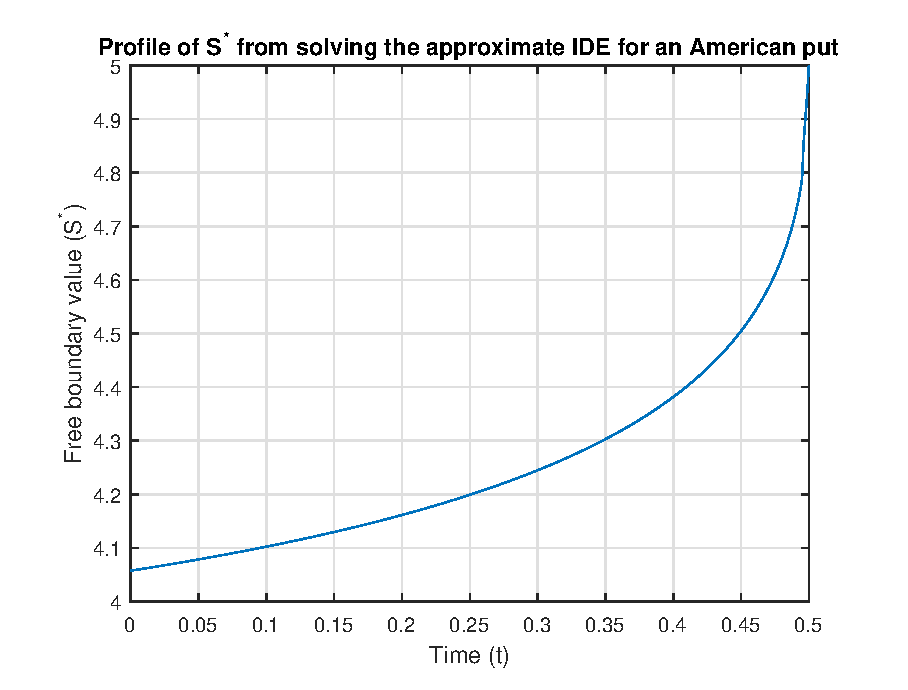
\includegraphics[scale=0.8]{figures/SfreePut.eps}
		\caption{The profile for $S^*$ from solving the approximate IDE~\eqref{eqn:SApproxPutLN} using $t=0$, $T=0.5$, $K = 5$, $r=0.05$, $q=0$, and $\sigma = 0.3$. The associated lognormal parameters are $\mu_Y = 0.9$, $\sigma_Y = 0.45$, and $\lambda = 0.1$.}
		\label{fig:amerputFreeBoundary}
	\end{figure}

\subsection{Results}
Here we will report the numerical outcomes from solving~\eqref{eqn:amerputjumpLNApprox} paired with solving the system for $S^*$~\eqref{eqn:SApproxPutLN}, \eqref{eqn:freePutTLN} against the FDM~\eqref{eqn:FDMPIDE}. Similar to the plot for $S^*$ that was displayed in the previous section, we will be employing the exact same parameter values. The financial parameters we will be using are $t=0$, $T=0.5$, $K = 5$, $r=0.05$, $q=0$, and $\sigma = 0.3$. The domain of $S_0$ (the underlying asset) will range from $10^{-3}$ to $4K$. This is done to emulate the scenarios of $S_0 \rightarrow 0$ and $S_0 \rightarrow \infty$. The jump-diffusion parameters are $\mu_Y = 0.9$, $\sigma_Y = 0.45$, and $\lambda = 0.1$. The simulations are done using MATLAB.

For the FDM, we use 101 spatial nodes and 501 temporal gridpoints. Consequently, this means we will also require 501 values of $S^*$ between $t=0$ and $t=0.5$. The domain of $S_0 \in [10^{-3},4K]$ will need to be divided into 100 equally-spaced subintervals to correspond to the 101 gridpoints used in the FDM. This is to ensure all resultant plots are consistent in terms of the input values used. For an American put option, we also require the following boundary conditions
	$$
		v_0^n = K, \quad v_I^n = 0, \quad \text{for all } n = 0,1,\ldots,N,
	$$
which correspond to the American put option at $S_0 \rightarrow 0$ and $S_0 \rightarrow \infty$ respectively for all time values in the domain. The option value curves are given in Figure~\ref{fig:amerputPlot} along with the absolute error between the two for the entire $S_0$ region. The MATLAB code for the FDM, the approximate IDE for $S^*$, and solving~\eqref{eqn:amerputjumpLNApprox} is available in the appendix with comments on how the code functions. Specifically, Appendix C.3 contains all that was used in this chapter.
	\begin{figure}[!h]
		\centering
		\subfigure[American put prices under jump-diffusion dynamics solved using the FDM scheme~\eqref{eqn:FDMPIDE} compared against~\eqref{eqn:amerputjumpLNApprox} with~\eqref{eqn:SApproxPutLN},~\eqref{eqn:freePutTLN} for the free boundary $S^*$. The price domain for the underlying asset is $(10^{-3},4K)$. \label{fig:amerputComp}]{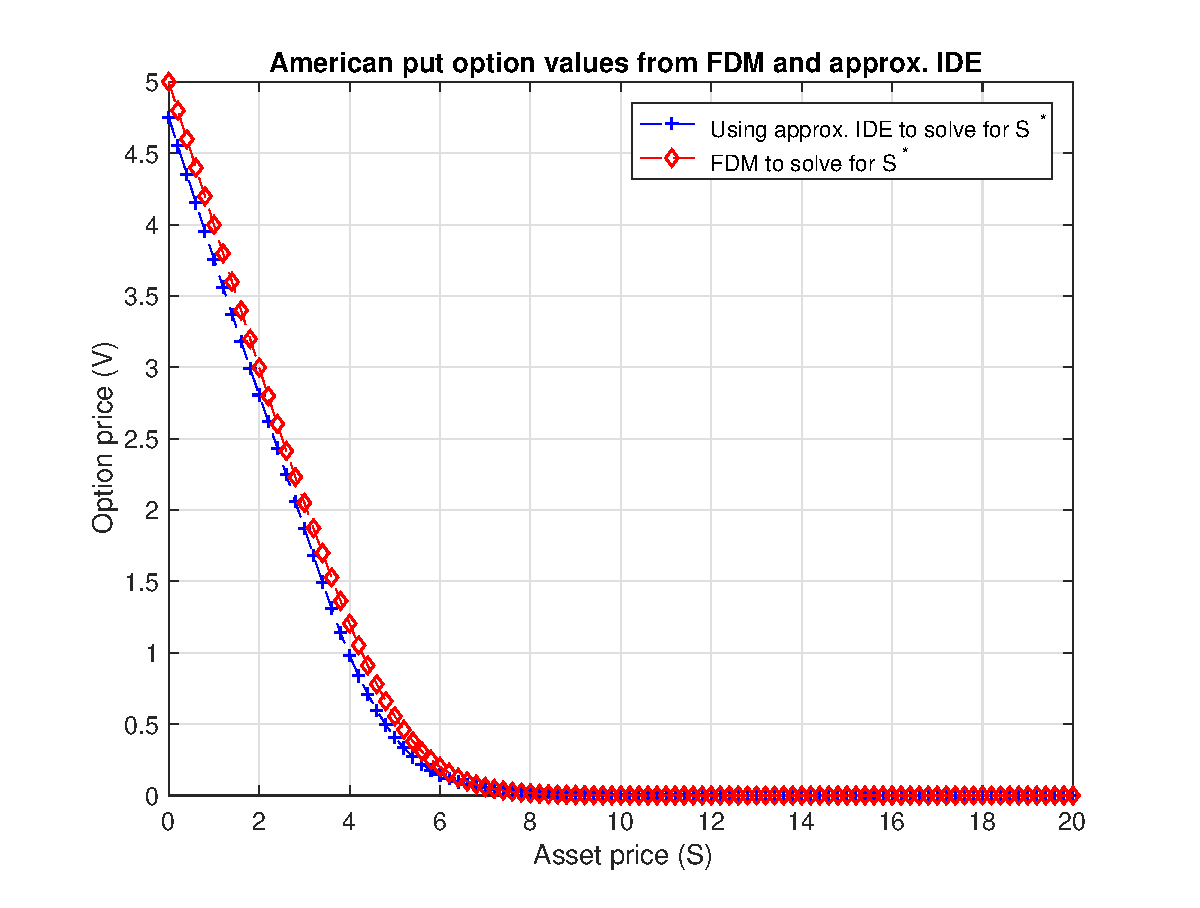
\includegraphics[width=0.7\linewidth]{figures/amerputFDMApprox.eps}\hspace*{3pt}}
		\subfigure[The absolute error between the FDM and using~\eqref{eqn:SApproxPutLN} for the American put values in a jump-diffusion model. \label{fig:amerputError}]{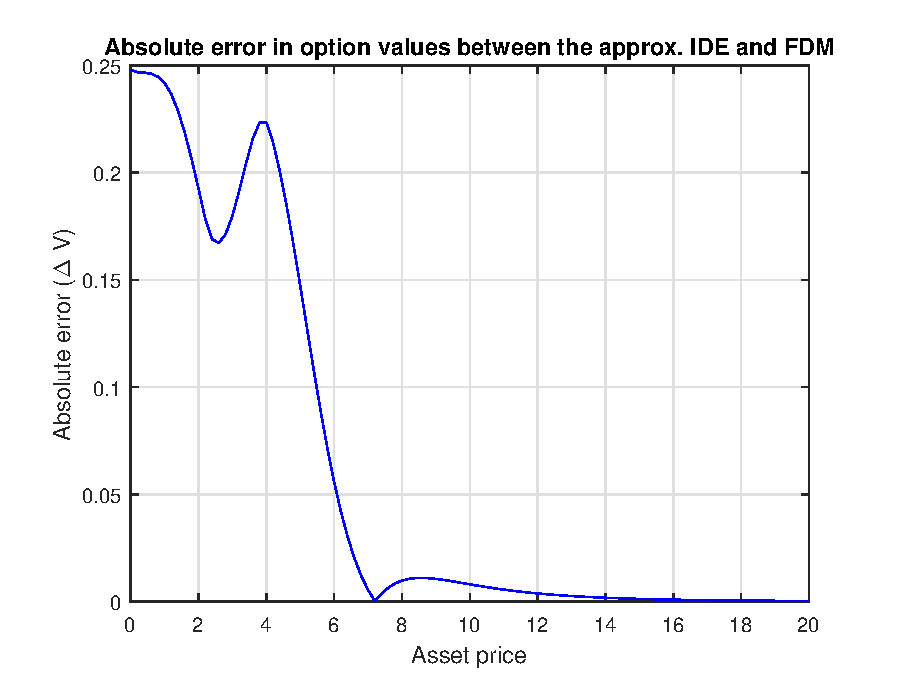
\includegraphics[width=0.7\linewidth]{figures/amerputFDMApproxError.eps}
			}
		\caption{American put value plots from the FDM and approximate IDE system using~\eqref{eqn:amerputjumpLNApprox},~\eqref{eqn:SApproxPutLN}, and~\eqref{eqn:freePutTLN}. The domain for the asset price is once again $(10^{-3},4K)$.}
		\label{fig:amerputPlot}
\end{figure}
 
From Figure~\ref{fig:amerputComp}, we can see that the American put option profiles overlap quite closely. Despite the assumptions that were made in order to simplify the pricing formula in~\eqref{eqn:amerputjumpLNApprox}, the errors that would have arose did not propagate to the resulting option values. This is highlighted in the absolute error between the option values in Figure~\ref{fig:amerputError} where the difference is only marginal.

\subsection{Conclusion}
In conclusion, we have derived an approximate IDE that enables us to solve for the optimal exercise boundary in a jump-diffusion model without the need to pair it with its corresponding option valuation formula. Furthermore, upon setting an approximate term for one of the integral terms for the American put option pricing formula, we were able to obtain an explicit approximation for the American put in jump-diffusion dynamics. The numerical reliability of these results were compared against the FDM to directly solve the Merton PIDE. Additionally the accuracy was acceptable for the given parameter values. Tentative future research could entail trialing different approximations for the integral term that appears in~\eqref{eqn:amerputjumpLNApprox} to make the pricing formula a better explicit approximate and also investigating the behaviour of such results when accounting for discrete dividend payments.